% **************************************************************************************************************
% A Classic Thesis Style
% An Homage to The Elements of Typographic Style
%
% Copyright (C) 2018 André Miede and Ivo Pletikosić
%
% If you like the style then I would appreciate a postcard. My address
% can be found in the file ClassicThesis.pdf. A collection of the
% postcards I received so far is available online at
% http://postcards.miede.de
%
% License:
% This program is free software; you can redistribute it and/or modify
% it under the terms of the GNU General Public License as published by
% the Free Software Foundation; either version 2 of the License, or
% (at your option) any later version.
%
% This program is distributed in the hope that it will be useful,
% but WITHOUT ANY WARRANTY; without even the implied warranty of
% MERCHANTABILITY or FITNESS FOR A PARTICULAR PURPOSE.  See the
% GNU General Public License for more details.
% **************************************************************************************************************
\RequirePackage{silence} % :-\
    \WarningFilter{scrreprt}{Usage of package `titlesec'}
    %\WarningFilter{scrreprt}{Activating an ugly workaround}
    \WarningFilter{titlesec}{Non standard sectioning command detected}
\documentclass[twoside,openright,titlepage,numbers=noenddot,%1headlines,
                headinclude,cleardoublepage=empty,abstract=on,
                BCOR=5mm,paper=a4,fontsize=11pt,dvipsnames
                ]{scrreprt}
\usepackage{listings}
\usepackage{color}

\usepackage{amsmath}
\usepackage{svg}
\usepackage{amssymb}
\usepackage{amsthm}
\usepackage{extarrows}
\usepackage[linesnumbered]{algorithm2e}
\newcommand{\func}[1]{{\fontfamily{kurierl}\selectfont \text{#1}}}
\newcommand{\funcfigure}[1]{{\fontfamily{kurierl}\selectfont \text{#1}}}


\definecolor{mygreen}{rgb}{0,0.6,0}
\definecolor{mygray}{rgb}{0.5,0.5,0.5}
\definecolor{mymauve}{rgb}{0.58,0,0.82}

\lstset{ 
  backgroundcolor=\color{white},   % choose the background color; you must add \usepackage{color} or \usepackage{xcolor}; should come as last argument
  basicstyle=\footnotesize,        % the size of the fonts that are used for the code
  breakatwhitespace=false,         % sets if automatic breaks should only happen at whitespace
  breaklines=true,                 % sets automatic line breaking
  captionpos=b,                    % sets the caption-position to bottom
  commentstyle=\color{mygreen},    % comment style
  deletekeywords={...},            % if you want to delete keywords from the given language
  escapechar=\%,          % if you want to add LaTeX within your code
  extendedchars=true,              % lets you use non-ASCII characters; for 8-bits encodings only, does not work with UTF-8
  firstnumber=1000,                % start line enumeration with line 1000
  frame=lines,	                   % adds a frame around the code
  keepspaces=true,                 % keeps spaces in text, useful for keeping indentation of code (possibly needs columns=flexible)
  keywordstyle=\color{red},       % keyword style
  language=Octave,                 % the language of the code
  morekeywords={*,...},            % if you want to add more keywords to the set
  numbers=left,                    % where to put the line-numbers; possible values are (none, left, right)
  stepnumber=1,
  numbersep=5pt,                   % how far the line-numbers are from the code
  numberstyle=\tiny\color{mygray}, % the style that is used for the line-numbers
  rulecolor=\color{black},         % if not set, the frame-color may be changed on line-breaks within not-black text (e.g. comments (green here))
  showspaces=false,                % show spaces everywhere adding particular underscores; it overrides 'showstringspaces'
  showstringspaces=false,          % underline spaces within strings only
  showtabs=false,                  % show tabs within strings adding particular underscores
  stringstyle=\color{mymauve},     % string literal style
  tabsize=2,	                   % sets default tabsize to 2 spaces
  title=\lstname                   % show the filename of files included with \lstinputlisting; also try caption instead of title
}
%********************************************************************
% Note: Make all your adjustments in here
%*******************************************************
% ****************************************************************************************************
% classicthesis-config.tex
% formerly known as loadpackages.sty, classicthesis-ldpkg.sty, and classicthesis-preamble.sty
% Use it at the beginning of your ClassicThesis.tex, or as a LaTeX Preamble
% in your ClassicThesis.{tex,lyx} with % ****************************************************************************************************
% classicthesis-config.tex
% formerly known as loadpackages.sty, classicthesis-ldpkg.sty, and classicthesis-preamble.sty
% Use it at the beginning of your ClassicThesis.tex, or as a LaTeX Preamble
% in your ClassicThesis.{tex,lyx} with % ****************************************************************************************************
% classicthesis-config.tex
% formerly known as loadpackages.sty, classicthesis-ldpkg.sty, and classicthesis-preamble.sty
% Use it at the beginning of your ClassicThesis.tex, or as a LaTeX Preamble
% in your ClassicThesis.{tex,lyx} with \input{classicthesis-config}
% ****************************************************************************************************
% If you like the classicthesis, then I would appreciate a postcard.
% My address can be found in the file ClassicThesis.pdf. A collection
% of the postcards I received so far is available online at
% http://postcards.miede.de
% ****************************************************************************************************


% ****************************************************************************************************
% 0. Set the encoding of your files. UTF-8 is the only sensible encoding nowadays. If you can't read
% äöüßáéçèê∂åëæƒÏ€ then change the encoding setting in your editor, not the line below. If your editor
% does not support utf8 use another editor!
% ****************************************************************************************************
\PassOptionsToPackage{utf8}{inputenc}
  \usepackage{inputenc}

\PassOptionsToPackage{T1}{fontenc} % T2A for cyrillics
  \usepackage{fontenc}


% ****************************************************************************************************
% 1. Configure classicthesis for your needs here, e.g., remove "drafting" below
% in order to deactivate the time-stamp on the pages
% (see ClassicThesis.pdf for more information):
% ****************************************************************************************************
\PassOptionsToPackage{
  drafting=false,    % print version information on the bottom of the pages
  tocaligned=false, % the left column of the toc will be aligned (no indentation)
  dottedtoc=true,  % page numbers in ToC flushed right
  eulerchapternumbers=true, % use AMS Euler for chapter font (otherwise Palatino)
  linedheaders=false,       % chaper headers will have line above and beneath
  floatperchapter=true,     % numbering per chapter for all floats (i.e., Figure 1.1)
  eulermath=false,  % use awesome Euler fonts for mathematical formulae (only with pdfLaTeX)
  beramono=true,    % toggle a nice monospaced font (w/ bold)
  palatino=true,    % deactivate standard font for loading another one, see the last section at the end of this file for suggestions
  style=classicthesis % classicthesis, arsclassica
}{classicthesis}


% ****************************************************************************************************
% 2. Personal data and user ad-hoc commands (insert your own data here)
% ****************************************************************************************************}

\newcommand{\myThesisType}{Bachelor's Thesis\xspace} % Master's Thesis
\newcommand{\myTitle}{Commit-Feature Interactions: Analyzing Structural and Dataflow Relations between Commits and Features\xspace}
\newcommand{\mySubtitle}{\xspace}
\newcommand{\myName}{Simon Steuer \xspace}
\newcommand{\myProf}{Prof. Dr. Sven Apel\xspace}
\newcommand{\myProfDepartment}{Chair of Software Engineering}
\newcommand{\myOtherProf}{Andreas Zeller\xspace}
\newcommand{\myOtherProfDepartment}{CISPA Helmholtz Center for Information Security}
\newcommand{\myAdvisor}{Sebastian Böhm\xspace}
\newcommand{\myAdvisorDepartment}{Chair of Software Engineering}
\newcommand{\myFaculty}{Saarland Informatics Campus\xspace}
\newcommand{\myDepartment}{Chair of Software Engineering\xspace}
\newcommand{\myUni}{Saarland University\xspace}
\newcommand{\myLocation}{Saarbrücken\xspace}
\newcommand{\mySubmissionDate}{\today\xspace}

\usepackage{datetime}
\newcommand{\myTime}{\monthname\xspace\the\year\xspace}
\newcommand{\myVersion}{\classicthesis}

% ********************************************************************
% Setup, finetuning, and useful commands
% ********************************************************************
\providecommand{\mLyX}{L\kern-.1667em\lower.25em\hbox{Y}\kern-.125emX\@}
\newcommand{\ie}{i.\,e.,}
\newcommand{\Ie}{I.\,e.,}
\newcommand{\eg}{e.\,g.,}
\newcommand{\Eg}{E.\,g.,}
% ****************************************************************************************************


% ****************************************************************************************************
% 3. Loading some handy packages
% ****************************************************************************************************
% ********************************************************************
% Packages with options that might require adjustments
% ********************************************************************
\PassOptionsToPackage{ngerman,american}{babel} % change this to your language(s), main language last
% Spanish languages need extra options in order to work with this template
%\PassOptionsToPackage{spanish,es-lcroman}{babel}
    \usepackage{babel}

\usepackage{csquotes}
\PassOptionsToPackage{%
  %backend=biber,bibencoding=utf8, %instead of bibtex
  backend=bibtex8,bibencoding=ascii,%
  language=auto,%
  style=numeric-comp,%
  %style=authoryear-comp, % Author 1999, 2010
  %bibstyle=authoryear,dashed=false, % dashed: substitute rep. author with ---
  sorting=nyt, % name, year, title
  maxcitenames=2, %default: 3, et al.
  maxbibnames=20, % default: 3, et al.
  %backref=true,%
  natbib=true % natbib compatibility mode (\citep and \citet still work)
}{biblatex}
    \usepackage{biblatex}

\PassOptionsToPackage{fleqn}{amsmath}       % math environments and more by the AMS
  \usepackage{amsmath}

% ********************************************************************
% General useful packages
% ********************************************************************
\usepackage{graphicx} %
\usepackage{scrhack} % fix warnings when using KOMA with listings package
\usepackage{xspace} % to get the spacing after macros right
\usepackage{acronym}
\usepackage{pdfpages}
% ****************************************************************************************************
%\usepackage{pgfplots} % External TikZ/PGF support (thanks to Andreas Nautsch)
%\usetikzlibrary{external}
%\tikzexternalize[mode=list and make, prefix=ext-tikz/]
% ****************************************************************************************************


% ****************************************************************************************************
% 4. Setup floats: tables, (sub)figures, and captions
% ****************************************************************************************************
\usepackage{tabularx} % better tables
% If you ever create tables: do it with booktabs
\usepackage{booktabs}
  \setlength{\extrarowheight}{3pt} % increase table row height
\newcommand{\tableheadline}[1]{\multicolumn{1}{l}{\spacedlowsmallcaps{#1}}}
\newcommand{\myfloatalign}{\centering} % to be used with each float for alignment
\usepackage{subfig}
% ****************************************************************************************************


% ****************************************************************************************************
% 5. Setup code listings
% ****************************************************************************************************
\usepackage{listings}
%\lstset{emph={trueIndex,root},emphstyle=\color{BlueViolet}}%\underbar} % for special keywords
\lstset{language=[LaTeX]Tex,%C++,
  morekeywords={PassOptionsToPackage,selectlanguage},
  keywordstyle=\color{RoyalBlue},%\bfseries,
  basicstyle=\small\ttfamily,
  %identifierstyle=\color{NavyBlue},
  commentstyle=\color{Green}\ttfamily,
  stringstyle=\rmfamily,
  numbers=none,%left,%
  numberstyle=\scriptsize,%\tiny
  stepnumber=5,
  numbersep=8pt,
  showstringspaces=false,
  breaklines=true,
  %frameround=ftff,
  %frame=single,
  belowcaptionskip=.75\baselineskip
  %frame=L
}
% ****************************************************************************************************




% ****************************************************************************************************
% 6. Last calls before the bar closes
% ****************************************************************************************************
% ********************************************************************
% Her Majesty herself
% ********************************************************************
\usepackage{classicthesis}


% ********************************************************************
% Fine-tune hyperreferences (hyperref should be called last)
% ********************************************************************
\hypersetup{%
  %draft, % hyperref's draft mode, for printing see below
  colorlinks=true, linktocpage=true, pdfstartpage=3, pdfstartview=FitV,%
  % uncomment the following line if you want to have black links (e.g., for printing)
  %colorlinks=false, linktocpage=false, pdfstartpage=3, pdfstartview=FitV, pdfborder={0 0 0},%
  breaklinks=true, pageanchor=true,%
  pdfpagemode=UseNone, %
  % pdfpagemode=UseOutlines,%
  plainpages=false, bookmarksnumbered, bookmarksopen=true, bookmarksopenlevel=1,%
  hypertexnames=true, pdfhighlight=/O,%nesting=true,%frenchlinks,%
  urlcolor=CTurl, linkcolor=CTlink, citecolor=CTcitation, %pagecolor=RoyalBlue,%
  %urlcolor=Black, linkcolor=Black, citecolor=Black, %pagecolor=Black,%
  pdftitle={\myTitle},%
  pdfauthor={\textcopyright\ \myName, \myUni, \myFaculty},%
  pdfsubject={},%
  pdfkeywords={},%
  pdfcreator={pdfLaTeX},%
  pdfproducer={LaTeX with hyperref and classicthesis}%
}


% ********************************************************************
% Setup autoreferences (hyperref and babel)
% ********************************************************************
% There are some issues regarding autorefnames
% http://www.tex.ac.uk/cgi-bin/texfaq2html?label=latexwords
% you have to redefine the macros for the
% language you use, e.g., american, ngerman
% (as chosen when loading babel/AtBeginDocument)
% ********************************************************************
\makeatletter
\@ifpackageloaded{babel}%
  {%
    \addto\extrasamerican{%
      \renewcommand*{\figureautorefname}{Figure}%
      \renewcommand*{\tableautorefname}{Table}%
      \renewcommand*{\partautorefname}{Part}%
      \renewcommand*{\chapterautorefname}{Chapter}%
      \renewcommand*{\sectionautorefname}{Section}%
      \renewcommand*{\subsectionautorefname}{Section}%
      \renewcommand*{\subsubsectionautorefname}{Section}%
    }%
    \addto\extrasngerman{%
      \renewcommand*{\paragraphautorefname}{Absatz}%
      \renewcommand*{\subparagraphautorefname}{Unterabsatz}%
      \renewcommand*{\footnoteautorefname}{Fu\"snote}%
      \renewcommand*{\FancyVerbLineautorefname}{Zeile}%
      \renewcommand*{\theoremautorefname}{Theorem}%
      \renewcommand*{\appendixautorefname}{Anhang}%
      \renewcommand*{\equationautorefname}{Gleichung}%
      \renewcommand*{\itemautorefname}{Punkt}%
    }%
      % Fix to getting autorefs for subfigures right (thanks to Belinda Vogt for changing the definition)
      \providecommand{\subfigureautorefname}{\figureautorefname}%
    }{\relax}
\makeatother

\definecolor{CTtitle}{named}{Blue}
\definecolor{CTurl}{named}{Blue}


% ********************************************************************
% Development Stuff
% ********************************************************************
\listfiles
%\PassOptionsToPackage{l2tabu,orthodox,abort}{nag}
%  \usepackage{nag}
%\PassOptionsToPackage{warning, all}{onlyamsmath}
%  \usepackage{onlyamsmath}


% ****************************************************************************************************
% 7. Further adjustments (experimental)
% ****************************************************************************************************
% ********************************************************************
% Changing the text area
% ********************************************************************
\areaset[current]{440pt}{686pt} % 686 (factor 2.2) + 33 head + 42 head \the\footskip
%\setlength{\marginparwidth}{7em}%
%\setlength{\marginparsep}{2em}%

% ********************************************************************
% Using different fonts
% ********************************************************************
%\usepackage[oldstylenums]{kpfonts} % oldstyle notextcomp
% \usepackage[osf]{libertine}
%\usepackage[light,condensed,math]{iwona}
%\renewcommand{\sfdefault}{iwona}
%\usepackage{lmodern} % <-- no osf support :-(
%\usepackage{cfr-lm} %
%\usepackage[urw-garamond]{mathdesign} <-- no osf support :-(
%\usepackage[default,osfigures]{opensans} % scale=0.95
%\usepackage[sfdefault]{FiraSans}
% \usepackage[opticals,mathlf]{MinionPro} % onlytext
% ********************************************************************
%\usepackage[largesc,osf]{newpxtext}
%\linespread{1.05} % a bit more for Palatino
% Used to fix these:
% https://bitbucket.org/amiede/classicthesis/issues/139/italics-in-pallatino-capitals-chapter
% https://bitbucket.org/amiede/classicthesis/issues/45/problema-testatine-su-classicthesis-style
% ********************************************************************
% ****************************************************************************************************

% ****************************************************************************************************
% If you like the classicthesis, then I would appreciate a postcard.
% My address can be found in the file ClassicThesis.pdf. A collection
% of the postcards I received so far is available online at
% http://postcards.miede.de
% ****************************************************************************************************


% ****************************************************************************************************
% 0. Set the encoding of your files. UTF-8 is the only sensible encoding nowadays. If you can't read
% äöüßáéçèê∂åëæƒÏ€ then change the encoding setting in your editor, not the line below. If your editor
% does not support utf8 use another editor!
% ****************************************************************************************************
\PassOptionsToPackage{utf8}{inputenc}
  \usepackage{inputenc}

\PassOptionsToPackage{T1}{fontenc} % T2A for cyrillics
  \usepackage{fontenc}


% ****************************************************************************************************
% 1. Configure classicthesis for your needs here, e.g., remove "drafting" below
% in order to deactivate the time-stamp on the pages
% (see ClassicThesis.pdf for more information):
% ****************************************************************************************************
\PassOptionsToPackage{
  drafting=false,    % print version information on the bottom of the pages
  tocaligned=false, % the left column of the toc will be aligned (no indentation)
  dottedtoc=true,  % page numbers in ToC flushed right
  eulerchapternumbers=true, % use AMS Euler for chapter font (otherwise Palatino)
  linedheaders=false,       % chaper headers will have line above and beneath
  floatperchapter=true,     % numbering per chapter for all floats (i.e., Figure 1.1)
  eulermath=false,  % use awesome Euler fonts for mathematical formulae (only with pdfLaTeX)
  beramono=true,    % toggle a nice monospaced font (w/ bold)
  palatino=true,    % deactivate standard font for loading another one, see the last section at the end of this file for suggestions
  style=classicthesis % classicthesis, arsclassica
}{classicthesis}


% ****************************************************************************************************
% 2. Personal data and user ad-hoc commands (insert your own data here)
% ****************************************************************************************************}

\newcommand{\myThesisType}{Bachelor's Thesis\xspace} % Master's Thesis
\newcommand{\myTitle}{Commit-Feature Interactions: Analyzing Structural and Dataflow Relations between Commits and Features\xspace}
\newcommand{\mySubtitle}{\xspace}
\newcommand{\myName}{Simon Steuer \xspace}
\newcommand{\myProf}{Prof. Dr. Sven Apel\xspace}
\newcommand{\myProfDepartment}{Chair of Software Engineering}
\newcommand{\myOtherProf}{Andreas Zeller\xspace}
\newcommand{\myOtherProfDepartment}{CISPA Helmholtz Center for Information Security}
\newcommand{\myAdvisor}{Sebastian Böhm\xspace}
\newcommand{\myAdvisorDepartment}{Chair of Software Engineering}
\newcommand{\myFaculty}{Saarland Informatics Campus\xspace}
\newcommand{\myDepartment}{Chair of Software Engineering\xspace}
\newcommand{\myUni}{Saarland University\xspace}
\newcommand{\myLocation}{Saarbrücken\xspace}
\newcommand{\mySubmissionDate}{\today\xspace}

\usepackage{datetime}
\newcommand{\myTime}{\monthname\xspace\the\year\xspace}
\newcommand{\myVersion}{\classicthesis}

% ********************************************************************
% Setup, finetuning, and useful commands
% ********************************************************************
\providecommand{\mLyX}{L\kern-.1667em\lower.25em\hbox{Y}\kern-.125emX\@}
\newcommand{\ie}{i.\,e.,}
\newcommand{\Ie}{I.\,e.,}
\newcommand{\eg}{e.\,g.,}
\newcommand{\Eg}{E.\,g.,}
% ****************************************************************************************************


% ****************************************************************************************************
% 3. Loading some handy packages
% ****************************************************************************************************
% ********************************************************************
% Packages with options that might require adjustments
% ********************************************************************
\PassOptionsToPackage{ngerman,american}{babel} % change this to your language(s), main language last
% Spanish languages need extra options in order to work with this template
%\PassOptionsToPackage{spanish,es-lcroman}{babel}
    \usepackage{babel}

\usepackage{csquotes}
\PassOptionsToPackage{%
  %backend=biber,bibencoding=utf8, %instead of bibtex
  backend=bibtex8,bibencoding=ascii,%
  language=auto,%
  style=numeric-comp,%
  %style=authoryear-comp, % Author 1999, 2010
  %bibstyle=authoryear,dashed=false, % dashed: substitute rep. author with ---
  sorting=nyt, % name, year, title
  maxcitenames=2, %default: 3, et al.
  maxbibnames=20, % default: 3, et al.
  %backref=true,%
  natbib=true % natbib compatibility mode (\citep and \citet still work)
}{biblatex}
    \usepackage{biblatex}

\PassOptionsToPackage{fleqn}{amsmath}       % math environments and more by the AMS
  \usepackage{amsmath}

% ********************************************************************
% General useful packages
% ********************************************************************
\usepackage{graphicx} %
\usepackage{scrhack} % fix warnings when using KOMA with listings package
\usepackage{xspace} % to get the spacing after macros right
\usepackage{acronym}
\usepackage{pdfpages}
% ****************************************************************************************************
%\usepackage{pgfplots} % External TikZ/PGF support (thanks to Andreas Nautsch)
%\usetikzlibrary{external}
%\tikzexternalize[mode=list and make, prefix=ext-tikz/]
% ****************************************************************************************************


% ****************************************************************************************************
% 4. Setup floats: tables, (sub)figures, and captions
% ****************************************************************************************************
\usepackage{tabularx} % better tables
% If you ever create tables: do it with booktabs
\usepackage{booktabs}
  \setlength{\extrarowheight}{3pt} % increase table row height
\newcommand{\tableheadline}[1]{\multicolumn{1}{l}{\spacedlowsmallcaps{#1}}}
\newcommand{\myfloatalign}{\centering} % to be used with each float for alignment
\usepackage{subfig}
% ****************************************************************************************************


% ****************************************************************************************************
% 5. Setup code listings
% ****************************************************************************************************
\usepackage{listings}
%\lstset{emph={trueIndex,root},emphstyle=\color{BlueViolet}}%\underbar} % for special keywords
\lstset{language=[LaTeX]Tex,%C++,
  morekeywords={PassOptionsToPackage,selectlanguage},
  keywordstyle=\color{RoyalBlue},%\bfseries,
  basicstyle=\small\ttfamily,
  %identifierstyle=\color{NavyBlue},
  commentstyle=\color{Green}\ttfamily,
  stringstyle=\rmfamily,
  numbers=none,%left,%
  numberstyle=\scriptsize,%\tiny
  stepnumber=5,
  numbersep=8pt,
  showstringspaces=false,
  breaklines=true,
  %frameround=ftff,
  %frame=single,
  belowcaptionskip=.75\baselineskip
  %frame=L
}
% ****************************************************************************************************




% ****************************************************************************************************
% 6. Last calls before the bar closes
% ****************************************************************************************************
% ********************************************************************
% Her Majesty herself
% ********************************************************************
\usepackage{classicthesis}


% ********************************************************************
% Fine-tune hyperreferences (hyperref should be called last)
% ********************************************************************
\hypersetup{%
  %draft, % hyperref's draft mode, for printing see below
  colorlinks=true, linktocpage=true, pdfstartpage=3, pdfstartview=FitV,%
  % uncomment the following line if you want to have black links (e.g., for printing)
  %colorlinks=false, linktocpage=false, pdfstartpage=3, pdfstartview=FitV, pdfborder={0 0 0},%
  breaklinks=true, pageanchor=true,%
  pdfpagemode=UseNone, %
  % pdfpagemode=UseOutlines,%
  plainpages=false, bookmarksnumbered, bookmarksopen=true, bookmarksopenlevel=1,%
  hypertexnames=true, pdfhighlight=/O,%nesting=true,%frenchlinks,%
  urlcolor=CTurl, linkcolor=CTlink, citecolor=CTcitation, %pagecolor=RoyalBlue,%
  %urlcolor=Black, linkcolor=Black, citecolor=Black, %pagecolor=Black,%
  pdftitle={\myTitle},%
  pdfauthor={\textcopyright\ \myName, \myUni, \myFaculty},%
  pdfsubject={},%
  pdfkeywords={},%
  pdfcreator={pdfLaTeX},%
  pdfproducer={LaTeX with hyperref and classicthesis}%
}


% ********************************************************************
% Setup autoreferences (hyperref and babel)
% ********************************************************************
% There are some issues regarding autorefnames
% http://www.tex.ac.uk/cgi-bin/texfaq2html?label=latexwords
% you have to redefine the macros for the
% language you use, e.g., american, ngerman
% (as chosen when loading babel/AtBeginDocument)
% ********************************************************************
\makeatletter
\@ifpackageloaded{babel}%
  {%
    \addto\extrasamerican{%
      \renewcommand*{\figureautorefname}{Figure}%
      \renewcommand*{\tableautorefname}{Table}%
      \renewcommand*{\partautorefname}{Part}%
      \renewcommand*{\chapterautorefname}{Chapter}%
      \renewcommand*{\sectionautorefname}{Section}%
      \renewcommand*{\subsectionautorefname}{Section}%
      \renewcommand*{\subsubsectionautorefname}{Section}%
    }%
    \addto\extrasngerman{%
      \renewcommand*{\paragraphautorefname}{Absatz}%
      \renewcommand*{\subparagraphautorefname}{Unterabsatz}%
      \renewcommand*{\footnoteautorefname}{Fu\"snote}%
      \renewcommand*{\FancyVerbLineautorefname}{Zeile}%
      \renewcommand*{\theoremautorefname}{Theorem}%
      \renewcommand*{\appendixautorefname}{Anhang}%
      \renewcommand*{\equationautorefname}{Gleichung}%
      \renewcommand*{\itemautorefname}{Punkt}%
    }%
      % Fix to getting autorefs for subfigures right (thanks to Belinda Vogt for changing the definition)
      \providecommand{\subfigureautorefname}{\figureautorefname}%
    }{\relax}
\makeatother

\definecolor{CTtitle}{named}{Blue}
\definecolor{CTurl}{named}{Blue}


% ********************************************************************
% Development Stuff
% ********************************************************************
\listfiles
%\PassOptionsToPackage{l2tabu,orthodox,abort}{nag}
%  \usepackage{nag}
%\PassOptionsToPackage{warning, all}{onlyamsmath}
%  \usepackage{onlyamsmath}


% ****************************************************************************************************
% 7. Further adjustments (experimental)
% ****************************************************************************************************
% ********************************************************************
% Changing the text area
% ********************************************************************
\areaset[current]{440pt}{686pt} % 686 (factor 2.2) + 33 head + 42 head \the\footskip
%\setlength{\marginparwidth}{7em}%
%\setlength{\marginparsep}{2em}%

% ********************************************************************
% Using different fonts
% ********************************************************************
%\usepackage[oldstylenums]{kpfonts} % oldstyle notextcomp
% \usepackage[osf]{libertine}
%\usepackage[light,condensed,math]{iwona}
%\renewcommand{\sfdefault}{iwona}
%\usepackage{lmodern} % <-- no osf support :-(
%\usepackage{cfr-lm} %
%\usepackage[urw-garamond]{mathdesign} <-- no osf support :-(
%\usepackage[default,osfigures]{opensans} % scale=0.95
%\usepackage[sfdefault]{FiraSans}
% \usepackage[opticals,mathlf]{MinionPro} % onlytext
% ********************************************************************
%\usepackage[largesc,osf]{newpxtext}
%\linespread{1.05} % a bit more for Palatino
% Used to fix these:
% https://bitbucket.org/amiede/classicthesis/issues/139/italics-in-pallatino-capitals-chapter
% https://bitbucket.org/amiede/classicthesis/issues/45/problema-testatine-su-classicthesis-style
% ********************************************************************
% ****************************************************************************************************

% ****************************************************************************************************
% If you like the classicthesis, then I would appreciate a postcard.
% My address can be found in the file ClassicThesis.pdf. A collection
% of the postcards I received so far is available online at
% http://postcards.miede.de
% ****************************************************************************************************


% ****************************************************************************************************
% 0. Set the encoding of your files. UTF-8 is the only sensible encoding nowadays. If you can't read
% äöüßáéçèê∂åëæƒÏ€ then change the encoding setting in your editor, not the line below. If your editor
% does not support utf8 use another editor!
% ****************************************************************************************************
\PassOptionsToPackage{utf8}{inputenc}
  \usepackage{inputenc}

\PassOptionsToPackage{T1}{fontenc} % T2A for cyrillics
  \usepackage{fontenc}


% ****************************************************************************************************
% 1. Configure classicthesis for your needs here, e.g., remove "drafting" below
% in order to deactivate the time-stamp on the pages
% (see ClassicThesis.pdf for more information):
% ****************************************************************************************************
\PassOptionsToPackage{
  drafting=false,    % print version information on the bottom of the pages
  tocaligned=false, % the left column of the toc will be aligned (no indentation)
  dottedtoc=true,  % page numbers in ToC flushed right
  eulerchapternumbers=true, % use AMS Euler for chapter font (otherwise Palatino)
  linedheaders=false,       % chaper headers will have line above and beneath
  floatperchapter=true,     % numbering per chapter for all floats (i.e., Figure 1.1)
  eulermath=false,  % use awesome Euler fonts for mathematical formulae (only with pdfLaTeX)
  beramono=true,    % toggle a nice monospaced font (w/ bold)
  palatino=true,    % deactivate standard font for loading another one, see the last section at the end of this file for suggestions
  style=classicthesis % classicthesis, arsclassica
}{classicthesis}


% ****************************************************************************************************
% 2. Personal data and user ad-hoc commands (insert your own data here)
% ****************************************************************************************************}

\newcommand{\myThesisType}{Bachelor's Thesis\xspace} % Master's Thesis
\newcommand{\myTitle}{Commit-Feature Interactions: Analyzing Structural and Dataflow Relations between Commits and Features\xspace}
\newcommand{\mySubtitle}{\xspace}
\newcommand{\myName}{Simon Steuer \xspace}
\newcommand{\myProf}{Prof. Dr. Sven Apel\xspace}
\newcommand{\myProfDepartment}{Chair of Software Engineering}
\newcommand{\myOtherProf}{Andreas Zeller\xspace}
\newcommand{\myOtherProfDepartment}{CISPA Helmholtz Center for Information Security}
\newcommand{\myAdvisor}{Sebastian Böhm\xspace}
\newcommand{\myAdvisorDepartment}{Chair of Software Engineering}
\newcommand{\myFaculty}{Saarland Informatics Campus\xspace}
\newcommand{\myDepartment}{Chair of Software Engineering\xspace}
\newcommand{\myUni}{Saarland University\xspace}
\newcommand{\myLocation}{Saarbrücken\xspace}
\newcommand{\mySubmissionDate}{\today\xspace}

\usepackage{datetime}
\newcommand{\myTime}{\monthname\xspace\the\year\xspace}
\newcommand{\myVersion}{\classicthesis}

% ********************************************************************
% Setup, finetuning, and useful commands
% ********************************************************************
\providecommand{\mLyX}{L\kern-.1667em\lower.25em\hbox{Y}\kern-.125emX\@}
\newcommand{\ie}{i.\,e.,}
\newcommand{\Ie}{I.\,e.,}
\newcommand{\eg}{e.\,g.,}
\newcommand{\Eg}{E.\,g.,}
% ****************************************************************************************************


% ****************************************************************************************************
% 3. Loading some handy packages
% ****************************************************************************************************
% ********************************************************************
% Packages with options that might require adjustments
% ********************************************************************
\PassOptionsToPackage{ngerman,american}{babel} % change this to your language(s), main language last
% Spanish languages need extra options in order to work with this template
%\PassOptionsToPackage{spanish,es-lcroman}{babel}
    \usepackage{babel}

\usepackage{csquotes}
\PassOptionsToPackage{%
  %backend=biber,bibencoding=utf8, %instead of bibtex
  backend=bibtex8,bibencoding=ascii,%
  language=auto,%
  style=numeric-comp,%
  %style=authoryear-comp, % Author 1999, 2010
  %bibstyle=authoryear,dashed=false, % dashed: substitute rep. author with ---
  sorting=nyt, % name, year, title
  maxcitenames=2, %default: 3, et al.
  maxbibnames=20, % default: 3, et al.
  %backref=true,%
  natbib=true % natbib compatibility mode (\citep and \citet still work)
}{biblatex}
    \usepackage{biblatex}

\PassOptionsToPackage{fleqn}{amsmath}       % math environments and more by the AMS
  \usepackage{amsmath}

% ********************************************************************
% General useful packages
% ********************************************************************
\usepackage{graphicx} %
\usepackage{scrhack} % fix warnings when using KOMA with listings package
\usepackage{xspace} % to get the spacing after macros right
\usepackage{acronym}
\usepackage{pdfpages}
% ****************************************************************************************************
%\usepackage{pgfplots} % External TikZ/PGF support (thanks to Andreas Nautsch)
%\usetikzlibrary{external}
%\tikzexternalize[mode=list and make, prefix=ext-tikz/]
% ****************************************************************************************************


% ****************************************************************************************************
% 4. Setup floats: tables, (sub)figures, and captions
% ****************************************************************************************************
\usepackage{tabularx} % better tables
% If you ever create tables: do it with booktabs
\usepackage{booktabs}
  \setlength{\extrarowheight}{3pt} % increase table row height
\newcommand{\tableheadline}[1]{\multicolumn{1}{l}{\spacedlowsmallcaps{#1}}}
\newcommand{\myfloatalign}{\centering} % to be used with each float for alignment
\usepackage{subfig}
% ****************************************************************************************************


% ****************************************************************************************************
% 5. Setup code listings
% ****************************************************************************************************
\usepackage{listings}
%\lstset{emph={trueIndex,root},emphstyle=\color{BlueViolet}}%\underbar} % for special keywords
\lstset{language=[LaTeX]Tex,%C++,
  morekeywords={PassOptionsToPackage,selectlanguage},
  keywordstyle=\color{RoyalBlue},%\bfseries,
  basicstyle=\small\ttfamily,
  %identifierstyle=\color{NavyBlue},
  commentstyle=\color{Green}\ttfamily,
  stringstyle=\rmfamily,
  numbers=none,%left,%
  numberstyle=\scriptsize,%\tiny
  stepnumber=5,
  numbersep=8pt,
  showstringspaces=false,
  breaklines=true,
  %frameround=ftff,
  %frame=single,
  belowcaptionskip=.75\baselineskip
  %frame=L
}
% ****************************************************************************************************




% ****************************************************************************************************
% 6. Last calls before the bar closes
% ****************************************************************************************************
% ********************************************************************
% Her Majesty herself
% ********************************************************************
\usepackage{classicthesis}


% ********************************************************************
% Fine-tune hyperreferences (hyperref should be called last)
% ********************************************************************
\hypersetup{%
  %draft, % hyperref's draft mode, for printing see below
  colorlinks=true, linktocpage=true, pdfstartpage=3, pdfstartview=FitV,%
  % uncomment the following line if you want to have black links (e.g., for printing)
  %colorlinks=false, linktocpage=false, pdfstartpage=3, pdfstartview=FitV, pdfborder={0 0 0},%
  breaklinks=true, pageanchor=true,%
  pdfpagemode=UseNone, %
  % pdfpagemode=UseOutlines,%
  plainpages=false, bookmarksnumbered, bookmarksopen=true, bookmarksopenlevel=1,%
  hypertexnames=true, pdfhighlight=/O,%nesting=true,%frenchlinks,%
  urlcolor=CTurl, linkcolor=CTlink, citecolor=CTcitation, %pagecolor=RoyalBlue,%
  %urlcolor=Black, linkcolor=Black, citecolor=Black, %pagecolor=Black,%
  pdftitle={\myTitle},%
  pdfauthor={\textcopyright\ \myName, \myUni, \myFaculty},%
  pdfsubject={},%
  pdfkeywords={},%
  pdfcreator={pdfLaTeX},%
  pdfproducer={LaTeX with hyperref and classicthesis}%
}


% ********************************************************************
% Setup autoreferences (hyperref and babel)
% ********************************************************************
% There are some issues regarding autorefnames
% http://www.tex.ac.uk/cgi-bin/texfaq2html?label=latexwords
% you have to redefine the macros for the
% language you use, e.g., american, ngerman
% (as chosen when loading babel/AtBeginDocument)
% ********************************************************************
\makeatletter
\@ifpackageloaded{babel}%
  {%
    \addto\extrasamerican{%
      \renewcommand*{\figureautorefname}{Figure}%
      \renewcommand*{\tableautorefname}{Table}%
      \renewcommand*{\partautorefname}{Part}%
      \renewcommand*{\chapterautorefname}{Chapter}%
      \renewcommand*{\sectionautorefname}{Section}%
      \renewcommand*{\subsectionautorefname}{Section}%
      \renewcommand*{\subsubsectionautorefname}{Section}%
    }%
    \addto\extrasngerman{%
      \renewcommand*{\paragraphautorefname}{Absatz}%
      \renewcommand*{\subparagraphautorefname}{Unterabsatz}%
      \renewcommand*{\footnoteautorefname}{Fu\"snote}%
      \renewcommand*{\FancyVerbLineautorefname}{Zeile}%
      \renewcommand*{\theoremautorefname}{Theorem}%
      \renewcommand*{\appendixautorefname}{Anhang}%
      \renewcommand*{\equationautorefname}{Gleichung}%
      \renewcommand*{\itemautorefname}{Punkt}%
    }%
      % Fix to getting autorefs for subfigures right (thanks to Belinda Vogt for changing the definition)
      \providecommand{\subfigureautorefname}{\figureautorefname}%
    }{\relax}
\makeatother

\definecolor{CTtitle}{named}{Blue}
\definecolor{CTurl}{named}{Blue}


% ********************************************************************
% Development Stuff
% ********************************************************************
\listfiles
%\PassOptionsToPackage{l2tabu,orthodox,abort}{nag}
%  \usepackage{nag}
%\PassOptionsToPackage{warning, all}{onlyamsmath}
%  \usepackage{onlyamsmath}


% ****************************************************************************************************
% 7. Further adjustments (experimental)
% ****************************************************************************************************
% ********************************************************************
% Changing the text area
% ********************************************************************
\areaset[current]{440pt}{686pt} % 686 (factor 2.2) + 33 head + 42 head \the\footskip
%\setlength{\marginparwidth}{7em}%
%\setlength{\marginparsep}{2em}%

% ********************************************************************
% Using different fonts
% ********************************************************************
%\usepackage[oldstylenums]{kpfonts} % oldstyle notextcomp
% \usepackage[osf]{libertine}
%\usepackage[light,condensed,math]{iwona}
%\renewcommand{\sfdefault}{iwona}
%\usepackage{lmodern} % <-- no osf support :-(
%\usepackage{cfr-lm} %
%\usepackage[urw-garamond]{mathdesign} <-- no osf support :-(
%\usepackage[default,osfigures]{opensans} % scale=0.95
%\usepackage[sfdefault]{FiraSans}
% \usepackage[opticals,mathlf]{MinionPro} % onlytext
% ********************************************************************
%\usepackage[largesc,osf]{newpxtext}
%\linespread{1.05} % a bit more for Palatino
% Used to fix these:
% https://bitbucket.org/amiede/classicthesis/issues/139/italics-in-pallatino-capitals-chapter
% https://bitbucket.org/amiede/classicthesis/issues/45/problema-testatine-su-classicthesis-style
% ********************************************************************
% ****************************************************************************************************


%********************************************************************
% Bibliographies
%*******************************************************
\addbibresource{Bibliography.bib}

%********************************************************************
% Hyphenation
%*******************************************************
%\hyphenation{put special hyphenation here}

\begin{document}
\frenchspacing
\raggedbottom
\selectlanguage{american} % american ngerman
%\renewcommand*{\bibname}{new name}
%\setbibpreamble{}
\pagenumbering{roman}
\pagestyle{plain}
%********************************************************************
% Frontmatter
%*******************************************************
%*******************************************************
% Titlepage
%*******************************************************
\begin{titlepage}
    %\pdfbookmark[1]{\myTitle}{titlepage}
    % if you want the titlepage to be centered, uncomment and fine-tune the line below (KOMA classes environment)
    \begin{center}
        \large

        \hfill

        \vfill

        \myThesisType

        \vfill

        \begingroup
           {\LARGE  \color{CTtitle}\spacedallcaps{\myTitle} \\ \bigskip}
        \endgroup

        \spacedlowsmallcaps{\myName}

        \vfill

        \mySubmissionDate

	\vfill

        Advisor:\\
        \begin{tabular}{c c}
                \myAdvisor & \myAdvisorDepartment
        \end{tabular}
        
        \vfill

        Examiners:\\
        \begin{tabular}{c c}
        	\myProf & \myProfDepartment\\
		\myOtherProf & \myOtherProfDepartment
        \end{tabular}
    
    	\vfill
    	\vfill

        \myDepartment \\
        \myFaculty \\
        \myUni \\ \bigskip
        \vfill

	        
\includegraphics[height=2.2cm]{gfx/se-logo.png} \hfill 
\includegraphics[height=2.2cm]{gfx/uni-logo.pdf}  \\ \medskip

        \vfill

    \end{center}
\end{titlepage}

\thispagestyle{empty}

\hfill

\vfill

\noindent\myName: \textit{\myTitle,} %\myDegree,
\textcopyright\ \myTime

%\bigskip
%
%\noindent\spacedlowsmallcaps{Supervisors}: \\
%\myProf \\
%\myOtherProf \\
%\mySupervisor
%
%\medskip
%
%\noindent\spacedlowsmallcaps{Location}: \\
%\myLocation
%
%\medskip
%
%\noindent\spacedlowsmallcaps{Time Frame}: \\
%\myTime

%\cleardoublepage%*******************************************************
% Dedication
%*******************************************************
\thispagestyle{empty}
\phantomsection
\pdfbookmark[1]{Dedication}{Dedication}

\vspace*{3cm}

\begin{center}
    \emph{Ohana} means family. \\
    Family means nobody gets left behind, or forgotten. \\ \medskip
    --- Lilo \& Stitch
\end{center}

\medskip

\begin{center}
    Dedicated to the loving memory of Rudolf Miede. \\ \smallskip
    1939\,--\,2005
\end{center}

%\cleardoublepage\include{FrontBackmatter/Foreword}
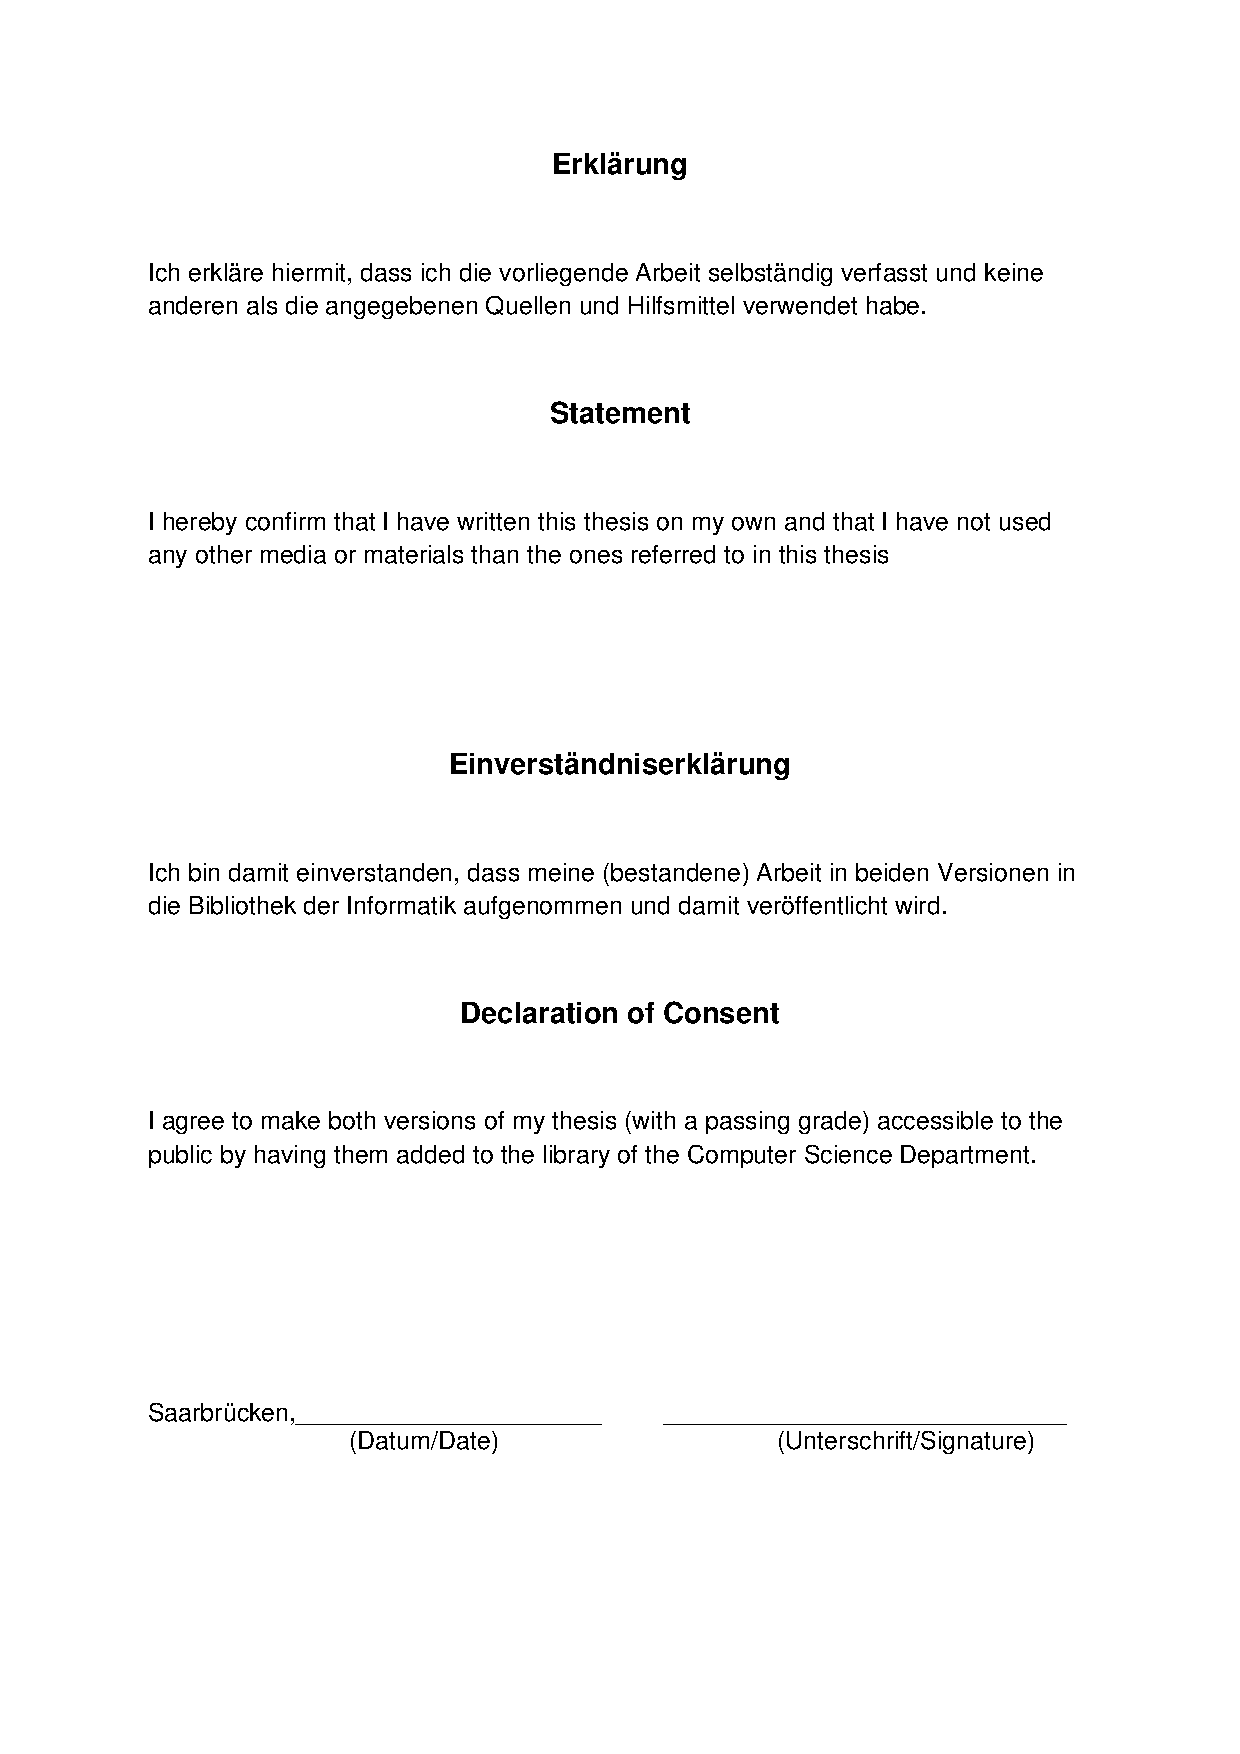
\includepdf{gfx/Selbstaendigkeitserklaerung_in_Arbeit_102016.pdf}
\cleardoublepage%*******************************************************
% Abstract
%*******************************************************
%\renewcommand{\abstractname}{Abstract}
\pdfbookmark[1]{Abstract}{Abstract}
% \addcontentsline{toc}{chapter}{\tocEntry{Abstract}}
\begingroup
\let\clearpage\relax
\let\cleardoublepage\relax
\let\cleardoublepage\relax

\chapter*{Abstract}

In software engineering, features play a pivotal role in implementing functionality of applications and adding configurability to them.
Their code is maintained in git repositories, where commits are used to introduce the latest source-code changes, thus gradually building the overall application and its features. % commits are an incremental unit of development
To allow for a deeper understanding of commits and features as well as their interplay, we connect both entities in the form of commit-feature interactions (CFIs).
For this, we extend the interaction analysis tool VaRA to implement the detection of structural and dataflow-based CFIs.
While the former provides information about the direct involvement of commits in developing features, the latter can uncover seemingly unrelated commits still influencing their functionality.

As previous studies have focused exclusively on interactions either among commits or among features, we are first to study interactions between the two entities. % we delve into research topics that neither can answer on their own,
We address research topics that neither can answer on their own, including insights into the development process of features and usage of commits therein. % , in particular we show use cases for the investigation of CFIs,
This enabled us, for instance, to confirm a derived best practice surrounding commits in feature development - namely, that commits should only change a single feature.
Furthermore, we find our employed dataflow analysis to be an essential part of gaining a complete overview of the interactions between commits and features in a project, as the majority of them take place only at dataflow level.
It should be noted that a substantial amount of dataflow occurs within or between features, and does not stem from other parts of a program.
That is, because commits constituting code of features have an almost certain chance of interacting with them via dataflow as well as a significantly increased probability of influencing other features. % this designates...

In this work, we also illustrate how CFIs can be applied to investigate an alternative albeit related form of interaction: author-feature interactions, achieved by mapping commits to their respective authors.
As some examined projects proved to be unfit for investigation on this topic, we were not able to conclusively answer our research questions here.
Nevertheless, we are convinced that this form of interaction promises to improve the understanding of developers on their interplay with features.
% based on the applications we have worked out

With this thesis, we accomplished an initial overview of commit-feature interactions, their use-cases as well as further applications and utilized them to determine dependencies between the involved entities. % the two involved entities

\vfill

\endgroup

\vfill

%\cleardoublepage%*******************************************************
% Publications
%*******************************************************
\pdfbookmark[1]{Publications}{publications}
\chapter*{Publications}\graffito{This is just an early --~and currently ugly~-- test!}
This might come in handy for PhD theses: some ideas and figures have appeared previously in the following publications:

%\noindent Put your publications from the thesis here. The packages \texttt{multibib} or \texttt{bibtopic} etc. can be used to handle multiple different bibliographies in your document.

\begin{refsection}[ownpubs]
    \small
    \nocite{*} % is local to to the enclosing refsection
    \printbibliography[heading=none]
\end{refsection}

\emph{Attention}: This requires a separate run of \texttt{bibtex} for your \texttt{refsection}, \eg, \texttt{ClassicThesis1-blx} for this file. You might also use \texttt{biber} as the backend for \texttt{biblatex}. See also \url{http://tex.stackexchange.com/questions/128196/problem-with-refsection}.

%\cleardoublepage%*******************************************************
% Acknowledgments
%*******************************************************
\pdfbookmark[1]{Acknowledgments}{acknowledgments}

\begin{flushright}{\slshape
    We have seen that computer programming is an art, \\
    because it applies accumulated knowledge to the world, \\
    because it requires skill and ingenuity, and especially \\
    because it produces objects of beauty.} \\ \medskip
    --- \defcitealias{knuth:1974}{Donald E. Knuth}\citetalias{knuth:1974} \citep{knuth:1974}
\end{flushright}



\bigskip

\begingroup
\let\clearpage\relax
\let\cleardoublepage\relax
\let\cleardoublepage\relax
\chapter*{Acknowledgments}
Put your acknowledgments here.

Many thanks to everybody who already sent me a postcard!

Regarding the typography and other help, many thanks go to Marco
Kuhlmann, Philipp Lehman, Lothar Schlesier, Jim Young, Lorenzo
Pantieri and Enrico Gregorio\footnote{Members of GuIT (Gruppo
Italiano Utilizzatori di \TeX\ e \LaTeX )}, J\"org Sommer,
Joachim K\"ostler, Daniel Gottschlag, Denis Aydin, Paride
Legovini, Steffen Prochnow, Nicolas Repp, Hinrich Harms,
Roland Winkler, Jörg Weber, Henri Menke, Claus Lahiri,
Clemens Niederberger, Stefano Bragaglia, Jörn Hees,
Scott Lowe, Dave Howcroft, Jos\'e M. Alcaide, David Carlisle,
Ulrike Fischer, Hugues de Lassus, Csaba Hajdu, Dave Howcroft, 
and the whole \LaTeX-community for support, ideas and
some great software.

\bigskip

\noindent\emph{Regarding \mLyX}: The \mLyX\ port was intially done by
\emph{Nicholas Mariette} in March 2009 and continued by
\emph{Ivo Pletikosi\'c} in 2011. Thank you very much for your
work and for the contributions to the original style.


\endgroup

\cleardoublepage%*******************************************************
% Table of Contents
%*******************************************************
\pagestyle{scrheadings}
%\phantomsection
\pdfbookmark[1]{\contentsname}{tableofcontents}
\setcounter{tocdepth}{2} % <-- 2 includes up to subsections in the ToC
\setcounter{secnumdepth}{3} % <-- 3 numbers up to subsubsections
\manualmark
\markboth{\spacedlowsmallcaps{\contentsname}}{\spacedlowsmallcaps{\contentsname}}
\tableofcontents
\automark[section]{chapter}
\renewcommand{\chaptermark}[1]{\markboth{\spacedlowsmallcaps{#1}}{\spacedlowsmallcaps{#1}}}
\renewcommand{\sectionmark}[1]{\markright{\textsc{\thesection}\enspace\spacedlowsmallcaps{#1}}}
%*******************************************************
% List of Figures and of the Tables
%*******************************************************
\clearpage
% \pagestyle{empty} % Uncomment this line if your lists should not have any headlines with section name and page number
\begingroup
    \let\clearpage\relax
    \let\cleardoublepage\relax
    %*******************************************************
    % List of Figures
    %*******************************************************
    %\phantomsection
    %\addcontentsline{toc}{chapter}{\listfigurename}
    \pdfbookmark[1]{\listfigurename}{lof}
    \listoffigures

    \vspace{8ex}

    %*******************************************************
    % List of Tables
    %*******************************************************
    %\phantomsection
    %\addcontentsline{toc}{chapter}{\listtablename}
    \pdfbookmark[1]{\listtablename}{lot}
    \listoftables

    \vspace{8ex}
    % \newpage

    %*******************************************************
    % List of Listings
    %*******************************************************
    %\phantomsection
    %\addcontentsline{toc}{chapter}{\lstlistlistingname}
    \pdfbookmark[1]{\lstlistlistingname}{lol}
    \lstlistoflistings

    \vspace{8ex}

    %*******************************************************
    % Acronyms
    %*******************************************************
    %\phantomsection
    \pdfbookmark[1]{Acronyms}{acronyms}
    \markboth{\spacedlowsmallcaps{Acronyms}}{\spacedlowsmallcaps{Acronyms}}
    \chapter*{Acronyms}
    \begin{acronym}[UMLX]
        \acro{DRY}{Don't Repeat Yourself}
        \acro{IDE}{Integrated Development Environment}
        \acro{UML}{Unified Modeling Language}
    \end{acronym}

\endgroup

%********************************************************************
% Mainmatter
%*******************************************************
\cleardoublepage
\pagestyle{scrheadings}
\pagenumbering{arabic}
%\setcounter{page}{90}
% use \cleardoublepage here to avoid problems with pdfbookmark
\cleardoublepage
%************************************************
\chapter{Introduction}\label{ch:introduction}
%************************************************

Features play an important part in modern programming, which shows in program paradigms such as feature-oriented software development (FOSD), where they are used to implement specific functionalities, can be activated or deactivated and thus add configurability to software systems.
As commits are used to contribute new source-code to a repository, it follows that commits can participate in the development of features by introducing source-code implementing their functionality. 
Furthermore, seemingly unrelated code that was changed or added by commits can influence soure-code of a feature through dataflow.
The described occurences in a program are structural and dataflow-based commit-feature interactions (CFIs), which we investigate in this work and provide insights into. 

Within a program, there exist many different abstract entities, such as commits and features, each serving different responsibilites.
For a better understanding of them, it is advantageous to know how these entities interact amongst themselves and with each other.
In the context of CFIs, bugs occuring in a feature could be linked to the latest commit affecting data of said feature, and consequently the author of the commit causing these bugs.
Especially for dataflow spanning over multiple files and many lines of code, it is often difficult or impossible to determine the respective interactions by studying the program oneself.
To enable an automatic detection of these interactions and allow for a complete overview of them inside a software project, Sattler created the interaction analysis tool VaRA~\cite{VaRA2023}.

In a prior study, \citet{sattler2023seal} used VaRA to examine interactions between commits showing that research on this topic can be applied to improve many aspects of software development.
For example, their research allowed for a deeper understanding of interactions between developers by linking commit interactions to their respective authors~\cite{sattler2023seal}. 
Similarly to commit interactions, internal feature interactions are dependencies between features at source-code level. 
While they have been the topic of some studies~\cite{kolesnikov2017relation}, the main intention was to utilize them as a predictor for external, e.g. performance interactions~\cite{siegmund2012predicting} of features.

Similarly to this thesis, previous studies have also investigated interactions between commits and features, particularly structural interactions to gain insights on the life cycle of features. 
There, \citet{michelon2021lifecycle} found that features are frequently changed by commits, including substantial modifications to their code, motivating that structural CFIs are a research topic worthy of further investigation.
A major difference between their and our work is that we examine projects where features are implemented via run-time configuration variables, while their research has focused on projects where variability is implemented through the C Preprocessor.
Not only does our method allow for the investigation of a new set of projects, but they way features are implemented might also be different for them.
% Besides that, our work also qualifies as unqiue and novel as we, 
To the best of our knowledge, we are the first to investigate dataflow interactions between commits and features.
Specifically, we speak of dataflow-based CFIs when there exists dataflow from the code representations of commits to that of features.
Thus, commits of these interactions introduced changes in the program affecting data which is later used inside a feature.
CFIs based on dataflow examine the program on a deeper level, allowing us to detect additional interactions missed by structural CFIs.
By combining dataflow-based and structural interactions, we can specify whether dataflow stems from outside or from inside the code constituting a feature, thus producing more informative data.

In a second analysis step, we follow the discussed approach of Sattler et al. by enriching CFIs with high-level repository information~\cite{sattler2023seal}.
In the same way in which we examine the influence of commits on features, we can examine how the authors contributing these commits interact with features.
As with commits, developers can affect features structurally or through dataflow.
There are some important differences though, as a developer can be the author of multiple commits, which can in turn affect features in different ways.
Thus, developers implementing features might also be the ones contributing changes located outside of feature-code, influencing them through dataflow.

\section{Goal of this Thesis}

The primary focus of this thesis is to gain an overview of how commits interact with features in software projects. 
Our goal is to lay basic groundwork regarding this subject that can be used in future research. 
As previously mentioned, we investigate two types of commit-feature interactions, namely structural and dataflow-based CFIs. 
Using structural CFIs, we aim to reveal insights about the development process of features and usage of commits therein. 
We also investigate to what extend our dataflow analysis can reveal interactions that cannot be discovered with a purely syntactical analysis.
By examining the interplay between the two types of CFIs, we hope to establish dependencies that will be considered in future studies.
Finally, we provide first insights on the interactions of authors with features to incentivize that this subject could be worthy of further investigation.

\section{Overview}

\autoref{ch:background} serves as an introduction to the concepts of code regions and interaction analyses, which are necessary to properly define structural and dataflow-based CFIs.
In \autoref{ch:example_chapter}, we give a definition of the two types of CFIs and dicuss their meaning in software projects as well as our \nameref{ch:implementation} of their detection in VaRA.
We also define properties surrounding features and commits, that are used in the following chapters, like the size of a feature~(\autoref{sec:feature_size}) and the feature-related concerns of a commit~(\autoref{sec:commit_concerns}).
The three research questions of this paper are established in \autoref{ch:methodology}, in which we also explain their operationalization.
The first RQ focuses on structural CFIs, the second RQ on dataflow-based CFIs and the last RQ on how authors interact with features.
\autoref{ch:evaluation} includes a detailed description of our results for the three posed research questions, followed by a separate discussion of the findings for each RQ. % containing background information and possible reasons for them.
In the last section of \autoref{ch:evaluation}, we address potential internal and external \hyperref[sec:threats]{Threats to the Validtiy} of this work.
In \autoref{ch:related_work}, we summarize previous studies investigating interactions inbetween commits and inbetween features.
We also cover topics such as the detection methods of feature-code and previous research on feature development. % to be done 
We summarize our results as well as their discussion and formulate thoughts adressing future research in \autoref{ch:conclusion}.





\cleardoublepage
%************************************************
\chapter{Background}\label{ch:background}
%************************************************

In this section, we summarize previous research on the topic of code regions and interaction analysis.
Thereby we give defintions of terms and dicuss concepts that are fundamental to our work.
In the next chapter, we use the introduced definitions and concepts to explain and investigate structural as well as dataflow-based commit-feature interactions.

\section{Code Regions}\label{ch:code_regions}
Software Programs consist of source code lines that are translated into an intermediate representation (IR) upon compilation.
IR accurately represents the source-code information and is utilized in many code improvement and transformation techniqes such as code-optimization.
Furthermore, static program analyses are conducted on top of IR or some sort of representation using IR. \\
Code regions are comprised of IR instructions that are consecutive in their control-flow. 
They are used to represent abstract entities of a software project, such as commits and features.
For this, each code region carries some kind of variability information, detailing its meaning.
It should be noted that there can be several code regions with the same meaning scattered across the program.
We dicuss two kinds of variablity information, namely commit and feature variability information, allowing us to define two separate code regions. \\
Commits are used within a version control system to represent the latest source code changes in its respective repository.
Inside a repository revision, a commit encompasses all source code lines that were added or last changed by it. 

\newtheorem{definition}{Definition}
\begin{definition}[commit regions]\label{def:commit_regions}
	\emph{The set of all consecutive instructions, that stem from source code lines belonging to a commit, is called a} commit region.
\end{definition}

As the source code lines changed by a commit are not necessarily contigious,
a commit can have many commit regions inside a program. 
To properly address the entire set of these commit regions within a program, we introduce the term regions of a commit.
We say that the \emph{regions of a commit} are the set of all commit regions that stem from source code lines of the commit. \\

In general, features are program parts implementing specific functionality.
In this work we focus on features that are modelled with the help of configuration variables that specify whether the functionality of a feature should be active or not.
Inside a program, configuration variables decide whether instructions, performing a feature's intended functionality, get executed. 
Detecting these control-flow dependencies is achieved by deploying extended static taint analyses, such as Lotrack\cite{lillack2014tracking}.

\begin{definition}[feature regions]\label{def:feature_regions}
	\emph{The set of all consecutive instructions, whose execution depends on a configuration variable belonging to a feature, is called a} feature region. 
\end{definition}

Similarly to commits, features can have many feature regions inside a program
as the instructions implementing their functionalities can be scattered across the program.
Here, we also say that the \emph{regions of a feature} are the set of all feature regions that stem from a feature's configuration variable. 

\section{Interaction Analysis}\label{sec:interaction_analysis}

In the previous chapter, we have already shown how different abstract entities of a software project, such as features and commits, can be assigned concrete representations within a program.
We can use interaction analyses to infer interactions between them by computing interactions between their concrete representations.
This can improve our understanding of them and give us insights on how they are used inside software projects. 
An important component of computing interactions between code regions is the concept of interaction relations between them introduced by \citet{sattler2023thesis}.
As we investigate structural and dataflow-based interactions, we make use of structural interaction ($\circledcirc$) and dataflow interaction ($\rightsquigarrow$) relations in this work. \\
The structural interaction relation between two code regions $r_1$ and $r_2$ is defined as follows:

\begin{definition}[structural interaction relation]\label{def:structural_relation}
	\emph{The interaction relation $r_1 \circledcirc r_2$ evaluates to true if at least one instruction that is part of $r_1$
	is also part of $r_2$.}
\end{definition}

The dataflow interaction relation between two code regions $r_1$ and $r_2$ is defined as:

\begin{definition}[dataflow interaction relation]\label{def:dataflow_relation}
	\emph{The interaction relation $r_1 \rightsquigarrow r_2$ evaluates to true if the data produced by at least one instruction i that is part of $r_1$
	flows as input to an instruction $i'$ that is part of $r_2$.}
\end{definition}

Essential to the research conducted in this paper is the interaction analysis created by Sattler~\cite{sattler2023thesis}.
Their interaction analysis tool VaRA is implemented on top of LLVM and PhASAR.
In their novel approach SEAL\cite{sattler2023seal}, VaRA is used to determine dataflow interactions between commits.
This is accomplished by computing dataflow interactions between the respective regions of commits.
Their approach for this will be shortly discussed here, however we advice their paper for a more thorough explanation. \\
The first step of their approach is to annonate code by mapping information about its regions to the compiler's intermediate representation.
This information is added to the LLVM-IR instructions during the construction of the IR.
In their paper, \citet{sattler2023seal} focus on commit regions, which contain information about the commit's hash and its respective repository.
The commit region of an instruction is extracted from the commit that last changed the source code line the instruction stems from.
Determining said commit is accomplished by accessing repository meta-data. \\
The second analysis step involves the actual computation of the interactions.
For this, Sattler et al. implemented a special, inter-procedural taint analysis.
It's able to track data flows between the commit regions of a given target program.
For this, information about which commit region affected it, is mapped onto data and tracked along program flow.
In this context, we would like to introduce the concept of taints, specifically commit taints.
Taints are used to to give information about which code regions have affected an instruction through dataflow.
For example, an instruction is tainted by a commit if its taint stems from a commit region.
It follows, that two commits, with their respective commit regions $r_1$ and $r_2$, interact through dataflow, when an instruction is part of one's commit region, $r_2$, while being tainted by $r_1$.
Consequently data produced by the commit region $r_1$ flows as input to an instruction within the commit region $r_2$, matching the \lowercase{\text{\nameref{def:dataflow_relation}}}.


%************************************************
\chapter{Commit-Feature Interactions}\label{ch:example_chapter}
%************************************************

In this section, we define structural and dataflow-based commit-feature interactions as well as properties related to them.
Furthermore, their meaning and relationship inside a software project is explained here. 
In the \nameref{ch:background} chapter, we discussed what purpose commits and features serve in a software project.
Commits are used to add new changes, whereas features are cohesive entities in a program implementing a specific functionality.
In this work, structural interactions are used to investigate how commits implement features and their functionality.
In addition, dataflow interactions are examined to gain additional knowledge on how new changes to a program, in the form of commits, affect features. 

\section{Structural CFIs}\label{sec:structural_cfis}

In the background chapter, we dicussed the concept of \nameref{ch:code_regions}, especially commit and feature regions. 
Logically, we speak of structural interactions between features and commits when their respective regions structurally interact. 
This structural interaction between code regions occurs when at least one instruction is part of both regions.
This is the case when code regions structurally interact through the \nameref{def:structural_relation} ($\circledcirc$).

\begin{definition}\label{def:structural_cfi}
\emph{A commit C with its commit regions $r_{1C}$, $r_{2C}$,... and a feature F with its feature regions $r_{1F}$, $r_{2F}$,... structurally interact, if at least one commit region $r_{iC}$ and one feature region $r_{jF}$ structurally interact with each other, i.e. $r_{iC}$ $\circledcirc$ $r_{jF}$.}
\end{definition}

Structural CFIs carry an important meaning, namely that the commit of the interaction was used to implement or change functionality of the feature of said interaction.
This can be seen when looking at an instruction accounting for a structural interaction, as it is both part of a commit as well as a feature region.
From the definition of \nameref{def:commit_regions}, it follows that the instruction stems from a source-code line that was last changed by the region's respective commit. 
From the definition of \nameref{def:feature_regions}, we also know that the instruction implements functionality of the feature region's respective feature. 
Thus, the commit of a structural interaction was used to extend or change the code implementing the feature of that interaction.
Following this, we can say that the commits, a feature structurally interacts with, implement the entire functionality of the feature.
That is because each source-code line of a git-repository was introduced by a commit and can only belong to a single commit.
Thus every instruction, including those part of feature regions, is annotated by exactly one commit region. 

Knowing the commits used to implement a feature allows us to determine the authors that developed it.
This is made possible by simply linking the commits, a feature structurally interacts with, to their respective authors.
By determining the authors of a feature, we can achieve a deeper insight into its development than solely focusing on the commits that implemented it. 

\section{Dataflow-based CFIs}\label{sec:dataflow_cfis}

Determining which commits affect a feature through dataflow can reveal additional interactions between commits and features that cannot be discovered with a structural analysis.
Especially dataflows that span over multiple files and many lines of code might be difficult for a programmer to be aware of.
Employing VaRA's dataflow analysis, that is dicussed in section~\ref{ch:implementation}, facilitates the detection of these dataflow interactions. \\
Commit interactions based on dataflow were explained in the \nameref{sec:interaction_analysis} section and can be considered as precursors to dataflow-based commit-feature interactions.
Similarly to commits interacting with other commits through dataflow, commits interact with features through dataflow, when there exists dataflow from a commit to a feature region.
This means that data allocared or changed within a commit region flows as input to an instruction located inside a feature region.
This pattern can also be matched to the \nameref{def:dataflow_relation} ($\rightsquigarrow$) when defining dataflow-based commit-feature interactions.

\begin{definition}\label{def:dataflow_cfi}
\emph{A commit C with its commit regions $r_{1C}$, $r_{2C}$,... and a feature F with its feature regions $r_{1F}$, $r_{2F}$,... interact through dataflow, if at least one commit region $r_{iC}$ interacts with a feature region $r_{jF}$ through dataflow, i.e. $r_{iC}$ $\rightsquigarrow$ $r_{jF}$.}
\end{definition}

\begin{lstlisting}[language=C++, caption={This code example contains both structural as well as dataflow-based commit feature interactions.
Commit \texttt{fc3a17d} implements the functionality of \texttt{FeatureDouble} for this function.
It follows that a structural commit-feature interaction can be found between them, as their respective commit and feature regions structurally interact.
Commit \texttt{7edb283} introduces the variable \texttt{ret} that is later used inside the feature region of \texttt{FeatureDouble}. 
This accounts for a commit-feature interaction through dataflow, as data that was produced within a commit region is used as input 
by an instruction belonging to a feature region of \texttt{FeatureDouble} later on in the program.}, label=DescriptiveLabel]	
1. int calc(int val) {                             %\vartriangleright% %\texttt{d93df4a}%
2.    int ret = val + 5;                           %\vartriangleright% %\texttt{7edb283}%
3.    if (FeatureDouble) {                         %\vartriangleright% %\texttt{fc3a17d}%    %\vartriangleright% %FeatureDouble%
4.        ret = ret * 2;                           %\vartriangleright% %\texttt{fc3a17d}%    %\vartriangleright% %FeatureDouble%
5.    }                                            %\vartriangleright% %\texttt{fc3a17d}%    %\vartriangleright% %FeatureDouble%
6.    return ret;                                  %\vartriangleright% %\texttt{d93df4a}%   
7. }                                               %\vartriangleright% %\texttt{d93df4a}%   
\end{lstlisting}

\section{Combination of CFIs}\label{sec:combination_cfis}

When investigating dataflow-based CFIs, it is important to be aware of the fact that structural CFIs heavily coincide with them.
This means that whenever commits and features structurally interact, they are likely to interact through dataflow as well.
As our structural analysis has already discovered that these commits and features interact with each other, 
we are more interested in commit-feature interactions that can only be detected by a dataflow analysis.
That this relationship between structural and dataflow interactions exists becomes clear when looking at an instruction accounting for a structural CFI.
From definition~\ref{def:structural_cfi}, we know that the instruction belongs to a commit region of the interaction's respective commit.
It follows that data changed inside the instruction produces commit taints for instructions that use the data as input. 
Now, if instructions that use the data as input are also part of a feature region of the interaction's respective feature, the commit and feature of the structural interaction will also interact through dataflow.
However, such dataflow is very likely to occur, as features are functional units, whose instructions build and depend upon each other. 
Knowing this we can differentiate between dataflow-based CFIs that occur within the regions of a feature and those where data flows from outside the regions of a feature into it.
From prior explanations, it follows that this differentiation can be accomplished by simply checking whether a commit that influences a feature through dataflow, also structurally interacts with it. 

\section{Feature Size}\label{sec:feature_size}

When examining commit-feature interactions in a project, it is helpful to have a measure that can estimate the size of a feature.
We can use such a measure to compare features with each other and, thus, put the number of their interactions into perspective.
Considering our implementation, it makes most sense to define the size of a feature as the number of instructions implementing its functionality inside a program.
As the instructions inside the regions of a feature implement its functionality, we can the define the size of a feature as follows:
\begin{definition} \label{def:feature_size}
\emph{The} size \emph{of a feature is the number of instructions that are part of its feature regions.}
\end{definition}
It's possible to calculate the defined size of a feature by calculating the number of instructions in which structural CFIs occur.
That is, because every instruction that is part of a feature region accounts for a structural commit-feature interaction, as every instruction is part of exactly one commit region as shown in the beginning of this section.
It follows, that we do not miss any instructions that are part of feature regions and do not count any such instruction more than once. 

\section{Nesting Degree of Structural CFIs}\label{sec:nesting_degree}

In contrast to commit regions, multiple regions of different features can appear in a single instruction.
Here, we say that the number of feature regions inside an instruction equals its nesting degree.
With increasing nesting degree of an instruction, it becomes less certain which purpose the instruction serves specifically.
It could implement functionality of only a single feature present in the instruction's feature regions or any combination of them potentially.
For an instruction with a nesting degree of one, we can be most certain about its purpose, namely implementing the functionality of the one feature present in the instruction.
This observation also bears consequences in the way we look at and judge structural CFIs, as we can also define a nesting degree for them:
\begin{definition} \label{def:nesting_degree}
\emph{The} nesting degree \emph{of a structural CFI is the minimum nesting degrees of all instructions the interaction occurs in.}
\end{definition}
It follows that, if for example, a commit and a feature only structurally interact inside instructions with a nestig degree of two or higher, the nesting degree of their structural CFI is two.
If we now discover one more instruction, in which they interact structurally, and there is no other feature region present inside the instruction, their structural CFI's nesting degree will now be one. \\
The nesting degree of a structural CFI is a useful measure to estimate the likelihood for which a commit was used to specifically change or implement functionality of a feature.
We can be most certain for a structural CFI with nesting degree of one and become less certain for interactions with higher nesting degrees.

\section{Implementation}\label{ch:implementation}

The detection of structural as well as dataflow-based commit-feature interactions is implemented in VaRA \cite{VaRA2023}.
Additionaly to commit regions, VaRA maps information about its feature regions onto the compiler's IR during its construction.
Commit regions contain the hash and repository of their respective commits, whereas feature regions contain the name of the feature they originated from.
VaRA also gives us access to every llvm-IR instruction of a program and its attached information.
Thus, structural CFIs of a program can be collected by examining its compiled instructions.
According to definition~\ref{def:structural_cfi}, we can store a structural interaction between a commit and a feature, if an instruction is part of a respective commit and feature region.
For each such interaction we also save the number of instructions it occurs in. 
This is accomplished by incrementing its instruction counter if we happen to encounter a duplicate. 

With this, we are also able to calculate the size of a feature based on our collected structural CFIs and their respective instruction counters.
Following the explanations from section~\ref{sec:feature_size}, we can compute the size of a feature as the sum over the instruction counters of all found structural CFIs the feature is part of. 

In the \nameref{sec:interaction_analysis} section, we discussed the taint analysis deployed by VaRA.
There, VaRA computes information about which code regions have affected an instruction through dataflow.
Checking whether a taint stems from a commit region allows us to extract information about which commits have tainted an instruction.
Thus, dataflow-based commit-feature interactions can also be collected on instruction level.
According to definition~\ref{def:dataflow_cfi}, we can store a dataflow-based interaction between a commit and a feature, if an instruction has a respective commit taint while belonging to a respective feature region.
Consequently said instruction uses data, that was changed by a commit region earlier in the program, as its input, while belonging to a feature region. 

jetzt auch VaRA-TS erwähnen ??
\iffalse
For our research we examine numerous software projects to get a wide range of reference data, as commit-feature interactions could potentially vary greatly between different code spaces.
Accordingly, the VaRA-Tool-Suite was extended making it possible to generate a report comprising all found CFIs of an according type in a software project.
This aids us in examining several software projects to gain sufficient and sensible data about commit-feature interactions.
The created reports are also evaluated in the VaRA-Tool-Suite, which offers support to process and display statstics of the generated data. \\
\fi 

%************************************************
\chapter{Methodology}\label{ch:methodology}
%************************************************

The purpose of this chapter is to first formulate the research questions that we examine in our work
and then propose our method of answering them.

\section{Research Questions}\label{sec:research_questions}

In the \nameref{ch:example_chapter} chapter we dicussed the different meanings of structural and dataflow-based interactions.
With this knowledge, we can answer many interesting research topics. 
These topics include patterns in feature development and usage of commits therin as well as findings about how likely seemingly unrelated commits are to affect features inside a program.

\subsection*{\textbf{RQ1: How do commits and features structurally interact with each other?}}

We intend to research two main properties which already provide a lot of insight into the development process of features and best practices of commits therein.

\subsubsection*{Patterns around Feature Development}

Firstly, we examine the number of commits features interact with structurally. 
This gives us a direct estimate on how many commits were used in the development of a feature.
Our analysis also allows us to measure the size of feature, which can put the number of commits used to implement a feature into perspective.
We refine our investigation by factoring in the nesting degrees~\ref{sec:nesting_degree} of our collected structural CFIs.
This allows us to additionally determine the \textsf{definite} size of a feature showing us to what extent its code is nested inside other features.
Furthermore, we can differentiate between commits that most likely and those that only potentially implemented a feature's functionality.
By doing so, we intend to achieve a more accurate analysis regarding the number of commits used during a feature's development.

\subsubsection*{Usage of Commits in Feature Development}

Secondly, we examine how many features a commit interacts with structurally, i.e. how many features a commit usually changes. 
This is especially interesting when considering best practices surrounding the usage of commits.
It is preferred to keep commits atomic\cite{hundhausen2021commit_metrics} meaning they should only deal with a single concern.
As different features implement separate functionalities, it's unlikely for a commit to change several features while dealing with the same concern.
Transferring this to our work, high quality commits should mostly change a single feature.
Acquiring data on this issue might show how strictly this policy is enforced in the development of features across different projects. 
Here, differentiating between the nesting degrees of structural interactions provides us with more informative results. 
We can form a lower bound for the number of features a commit usually changes by only considering structural interactions with a nesting degree of one.
This way we only take into account commits for which we are certain that they were used to specifically implement a feature.
In our analysis, we should ideally filter commits whose purpose was refactoring code, since they do not fit our criteria of changing or adding functionality to a feature.
Exceptionally large commits might be best considered for this, as this is where we expect most commits used for large-scale refactoring to appear.
A qualitative review of these commits is still necessary to make a final decision on whether they should be filtered.

\subsection*{\textbf{RQ2: How do commits interact with features through dataflow?}}

Investigating dataflow inside a program can unveil interactions between its entities that were previously hidden from programmers.
This can help them understand the extent to which different parts of a program influence each other.
Furthermore, deploying the introduced analysis in a direct manner could ensure improvements in the daily life of a developer.
In the context of our work, an example for this could be the faciliation of finding the cause of and subsequently fixing bugs in features.
Bugs occuring in certain features could be traced back to the commits responsible for them by factoring in recent commits affecting said features through dataflow. \\
Previous studies have laid the groundwork for researching dataflow interactions between different abstract entities of a program.
While it has shown a wide range of interesting use-cases, it has focused solely on dataflow between commits.
That's why we aim to provide first insights into the properties of dataflow-based CFIs.
Specifically, we investigate how connected commits and features are by analyzing the number of features a commit affects through dataflow.
Knowing what fraction of all commits contributing code to a project are part of dataflow-based interactions can show how often new commits affect the data of a feature. 
Regarding this, it is worth considering the dependency dicussed in section \ref{sec:combination_cfis}, that structural interactions heavily coincide with dataflow interactions.
This implies that commits constituting code of a feature are very likely to influence said feature through dataflow as well.
In section \ref{sec:combination_cfis}, we also mention that the dataflow of commits not structurally interacting with a feature, must stem from outside the regions of the feature. 
Naturally, said dataflow is less intentional and subsequently more interesting, than dataflow occuring inside the regions of a feature. 
Programmers are less aware that changes introduced with these commits might affect the data of seemingly unrelated features.
Therefore, we intend to differentiate between dataflow interactions with an outside and those with an inside origin in our anaylsis.
This allows us to especially focus on commits part of outside dataflow interactions and examine their proportion among all commits. \\
Dataflow-based CFIs allow us to examine another interesting property, namely the number of commits affecting a feature through dataflow.
Here, we differentiate between commits \textsc{inside} and \textsc{outside} of features, i.e. commits that either do or don't contribute code to them.
We examine the proportion of outside to inside commits influencing a feature to gauge where most dataflow interactions of a feature stem from.
Considering our previous assumptions, the ratio of outside to inside commits could decrease with increasing size of a feature.
Smaller features are likely to structurally interact with less commits than their larger counterparts, resulting in them also interacting with less inside commits through dataflow.
However, the number of outside commits affecting data of a feature is not dependent on feature size in such a way.
This leads us to another relationship worth investigating, namely the relation between the size of a feature and the number of outside and inside commits interacting with it through dataflow.
We examine the two commit kinds separately, as we already have a strong supposition for inside commits, but are less certain for outside commits. 
Determining to what extent feature size is the driving factor in this relation, could tell us whether it is worth considering other possible properties of features in future analyses.

\subsection*{\textbf{RQ3: How do authors interact with features?}}

A simple yet promising way to extract more information out of the collected CFIs is to link the interaction's commits to their respective authors.
Thus, we are able to investigate how authors interact with features both structurally and through dataflow.
Similarly to the number of commits implementing a feature, we can now calculate the number of authors that participated in its development.
The same applies to commits interacting with features through dataflow, for which we can now determine the authors contributing these commits.
Here, we only consider outside commits, i.e. commits not constituting code of the feature, since we have already considered all inside commits when investigating the developers implementing a feature.
We are especially interested in how many authors exclusively interact with a feature through dataflow in comparison to the number of its developers.
This lets us determine whether the developers that implement features are also the ones mainly responsible for changes affecting them through dataflow. \\
Finally, we relate both types of author interactions to the respective size of a feature.
Regarding structural interactions, this allows us to determine whether a feature's extent in the source-code of a project is driving factor in the amount of authors needed to implement it. 
Software companies could use evidence on this issue as advice on how to allocate programmers on to-be implemented features.
Findings on the investigated dataflow interactions of authors could tell developers that their changes might affect small and, at first sight neglegible, features surprisingly often.
We also have a look at the specific functionality of features since their purpose could also play an important role in the number of authors interacting with it.

\begin{center}
\begin{tabular}{cc}
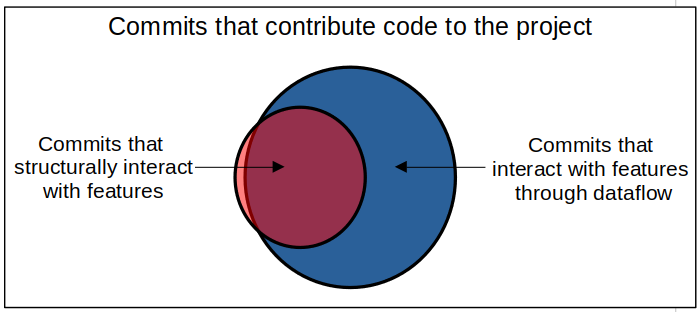
\includegraphics[height=6cm]{gfx/Commits-of-a-Software-Project.png}
\end{tabular}
\captionof{figure}{Illustration of different commit kinds}
\end{center}
\textsf{
In the first two \textbf{RQs} we have discussed different kinds of commits and the ways in which they interact with features. 
The above figure showcases them in a venn diagram and illustrates the dependencies and divisions between them.
}

\section{Operationalization}\label{sec:operationalization}

Here, we explain how the proposed RQs can be answered.
The general experiment process is the same for all RQs.
At first, we collect data comprimising all structural or dataflow-based CFIs by creating reports of a specific type for a chosen software project.
The collected data is then processed in order to gain information for each commit or feature in the project, such as the number of interacting commits and size of a feature.
The processed data is used to calculate statistical information, such as the mean and variance, or the strength of a correlation.
To facilitate a faster and better understanding of the processed data and calculated statistics, we display them graphically via bar or regression plots.
The projects we investigate in this work, for example \textsc{xz} and \textsc{gzip}, are of a small size and are used in a compression domain.
This choice is based on the fact, that our research intends to only lay basic groundwork, where smaller projects can already offer a lot of insight.
Since we only investigate a few projects, we chose them to be of a similar domain, such that a comparison between them makes more sense.
In the following sections, we explain our method of investigation in more detail for each RQ.

\subsection*{\textbf{RQ1: How do commits and features structurally interact with each other?}}

For this RQ, we examine the interactions contained in the structural reports created with our implementation in VaRA.
As there could be vast differences between the projects, we also work with and present their respective data separately.

\subsubsection*{Patterns around Feature Development}

From the collected structural reports, we first extract the number of structurally interacting commits and size for each feature.
For each interacting commit, we also determine the nesting degree of its structural interaction with the feature.
Additionally to the normal size of a feature, which we call \textsf{potential} size here, we calculate its \textsf{definite} size as well. 
The datapoints of the two properties are shown in two respective bar plots, where the values for each feature are shown in a separate bar.
The bars are labelled after the name of the feature they present, to allow for comparisons between the two plots and between different projects.
For comparisons between the investigated projects, we also calculate the average number of interacting commits and size of a feature for each project.
In the plot displaying the number of interacting commits, we stack the commits according to the nesting degree of their respective interaction with the feature.
The first part of each bar consists of commits interacting at a nesting degree of one, the second part of commits interacting at a higher nesting degree.
We do the same in the second plot, where the definite size forms the base of each bar upon which the difference with the potential size is added.
Logically, the stacked bars must be colored differently to see their respective distribution inside a feature.
The features are sorted in an increasing order according to the number of commits interacting at nesting degree one or their definite size.
Finally, we relate the two investigated properties in a \textsc{seaborn} regression plot.
Here, we show whether features increasing in size, in turn structurally interact with more commits, i.e. need more commits to be implemented.
Therefore, the value of the x-axis shows the size of a feature, whereas the y-axis shows the number of interacting commits.
Each feature is represented by a scatter point inside the plot combining its respective values from the two previous plots.
A linear regression line is drawn in the plot matching the occuring scatter points, where a rising graph could already indicate a positive correlation.
To check whether we are dealing with a statistically significant correlation, we compute the pearson correlation coefficient and its p-value in the \textsc{stats} submodule of the \textsc{scipy} python namespace.
To confirm our initial suspection of a strong positive correlation, the according correlation coefficient must be close to one, while the p-value must be close to zero falling below our rejection interval of 95\%.
Additionally to considering a dataset with the total number of interacting commits and size of a feature, we also consider a more restrictive dataset.
For this, we only relate the number of commits interacting at a nesting degree of one with the definite size of a feature.
It might be interesting to see whether only considering structural interactions and instructions with a nesting degree of one, could produce a stronger correlation.

\subsubsection*{Usage of Commits in Feature Development}

For each commit part of at least one structural interaction, we determine the number of features it structurally interacts with.
There, we also save at which nesting degree the commit and feature happen to interact with each other.
We ignore this property at first, although we will consider it in a later analysis step.
At first, we give a comprehensive overview of our initial results in a \textsc{seaborn} histplot for every investigated project.
The x-axis of the histogram shows the number of features a commit structurally interacts with, whereas the y-axis shows the number of commis for which the respective x-value matches.
If 50 commits structurally interact with a single feature inside a project, the y-value of one will be 50 accordingly.
Thus, we can quickly see to what extent our derived best practice surrounding commits in feature development is enforced in a project.
The more commits are located at one in comparison to other x-values, the more commits only change a single feature.
The histogram also shows us potential outlier commits, that structurally interact with a unusually many features.
To facilitate comparisons between projects, we choose the same x- and y-labels for every histogram. \\
In a second analysis step, we intend to further specify the broad overview shown in initial the plots.
As a baseline for the number of features a commit usually changes, we compute the average number of features a commit structurally interacts with in each project.
Following this, we now disregard structural interactions with a nesting degree of more than one. 
Thus, we only consider features for which we are relatively certain that the commit was used to implement or change their functionality.
Commits that exclusively interact with features at a high nesting degree, are now considered to change a single feature, as they could not be considered otherwise.
Furthermore, we filter exceptionally large commits, whose purpose we expect to be something else than implementing features, such as code-refactoring.
Similiarly to the regions of a commit, we determine its size in a repository as the number of source-code lines last changed or added by it.
We then apply tukey's fence with a k-value of 3 to filter far outliers of commit sizes.
Afterwards, we perform a qualitative review of the filtered commits to check whether our initial suspicion about their purpose was correct.
For both restrictions, we compute the average number of features changed, which should be lower than the calculated average without any restrictions.
Lastly, we combine both restrictions to form a final lower bound for the number of features a commit usually changes.
We show the four averages computed for each project in a cross-project table. 
By no means do we expect the actual average to be exactly at the final lower bound, but rather somewhere inbetween the final lower bound and the average with no restrictions.
That is because, we do not expect every structural interaction of a high nesting degree to be justifiably disregarded.

\subsection*{\textbf{RQ2: How do commits interact with features through dataflow?}}
an initial step of evaluating what fraction of commits affect features through dataflow, is first determining which set of commits we consider in our analysis \\
- logically, we should only consider commits that could potentially be part of a dataflow-based CFI \\
- the only prerequesite is for commits is to be represented by commit regions inside a program \\
The projects investigated for dataflow-based CFIs are the same projects as investigated for structural CFIs.
This choice gives us more insight into a single project and allows us to combine both analysis results as will be discussed below.
For this RQ, we consider all commits that currently contribute code to the repository, 
which we can extract from high level repository information of the project.
We process the collected data, such that, for each commit, we save how many features they interact with through dataflow.
Here, we also indicate whether a commit structurally interacts with a feature, which we can simply check by examining the according structural report.
With this information, we are able to separate commits into ones that implement parts of a feature and those that do not. 
We have already dicussed that commits used to implement a feature are much more likely to account for dataflow interactions.
We provide evidence for this by comparing the average amount of features the two types of commits affect through dataflow. 
Besides that we compute what fraction of commits have dataflow-based interactions with other features, once for all commits, once for commits that are part of a feature and once for commits that aren't part of a feature.
This shows how often commits affect features through dataflow based on their intended purpose, e.g. actively changing the functionality of a feature or changing something seemingly unrelated to a feature. 
With the data collected for each commit, we also plot the distribution of how many features they interact with.
This lets us recognize potential outliers, for example commits with much more dataflow interactions than the mean would suggest.
To check whether feature size is the driving factor in the number of outside commits affecting a feature through dataflow, we compute how strongly the two are correlated.
While we already know the size of each feature from RQ1, it's still neccesary to calculate, for each feature, which commits have dataflow-based interaction with them and subsequently filtering the commits that are part of a feature.

\subsection*{\textbf{RQ3: How do authors interact with features?}}

Here, we also examine the same projects as in the previous RQs.
That way we can reuse data produced in RQ1 to map each feature to the authors that implemented it.
For RQ1 we have already mapped each feature to the commits it interacts with, i.e. that contribute code to it.
It's possible to extract the authors of these commits by accessing high-level repository information.
This directly gives us the authors that implemented a feature.
With the processed data, we are able to calculate the average number of authors used to implement a feature and plot their distribution for a sound overview.
The size of each feature has also been calculated to answer the previous RQs.
With this information we aim to correlate the size of a feature with the amount of authors that implemented it in a regression analysis.

%************************************************
\chapter{Evaluation}\label{ch:evaluation}
%************************************************

This chapter evaluates the thesis core claims.
At first, we describe the results of our three RQs in \autoref{sec:results}.
Following this, we dicuss our results and to what extent they answer our posed research questions.
In \autoref{sec:threats}, we focus on internal and external threats to the validity of our findings and gathered data. 

\section{Results}\label{sec:results}

Here, we evaluate the results of each RQ separately. 
As in \autoref{ch:methodology}, we divide the first two RQs into two sub-sections each.
Most of our results are represented by plots with at least one figure containing them per RQ and sub-section.
Important statistical values of the examined projects, which we refer to in the text, are additionally shown in tables.

\subsection[RQ1]{Results: RQ1} 
\label{sec:eval:RQ1}

Examining the structural CFIs of different projects can give us insights into the patterns of feature development and the usage of commits therin.
We first generally desribe our results with the help of \autoref{fig:feature_sfbr_plot} and \autoref{fig:commit_sfbr_plot} as well as the tables \ref{tab:feature_sfbr_table} and \ref{tab:commit_sfbr_table}.
We also explain particularly interesting results of individual commits and features by investigating their specific purpose and properties.

\subsubsection*{Patterns of Feature Development}\label{sec:eval_feature_development}

In the first part of RQ1, we examine the number of commits involved in the development of a feature and relate it to its size.
Figure \ref{fig:feature_sfbr_plot} illustrates our results in three different plots for each project.
Each row displays the results for one project with the name of the respective project being shown on the far left. 
In the first column, we show the number of structurally interacting commits for each feature in a bar plot.
For all projects, we notice a wide distribution of structurally interacting commits between features.
Numerous features, across all projects, interact with less than $\math{5}$ commits suggesting that they need very little work to be implemented in comparison to other features.
Both \textsc{xz} and \textsc{lrzip} have features structurally interacting with more than $\math{20}$ commits, while \textsc{gzip} even has four features that interact with more than $\math{60}$ commits.
With a mean of 29, the features of \textsc{gzip} have by far the highest number of interacting commits on average.
\textsc{xz}, \textsc{lrzip} and \textsc{bzip2} have much lower averages at $\math{9}$, $\math{16}$ and $\math{4}$ respectively.
As all projects are of a compression domain, we can find several features with the same general functionality across the examined projects.
The \textsf{verbosity}-feature structurally interacts with the most commits in \textsc{xz} and \textsc{bzip2}, while the same is not the case for the \textsf{verbose}-feature of \textsc{gzip}.
Although \textsc{gzip} encompasses the highest average number of interacting commits, its \textsf{recursive}-feature only interacts with $\math{2}$ commits, while the \textsf{recursive}-feature of \textsc{lrzip} interacts with $\math{24}$ commits. 

In the second column of \autoref{fig:feature_sfbr_plot}, we display the calculated feature sizes for each project.
Again, we see a wide range of different feature sizes within all projects.
Most notabely, there are large jumps between adjacent features, for example from \textsf{to\_stdout} with a size of $\math{450}$ to \textsf{no\_name} with a size of $\math{7300}$ in \textsc{gzip}.
Similarly to the number of interacting commits, \textsc{gzip} has by far the highest average feature size at $\math{2500}$.
The average feature sizes for the other projects range from $\math{190}$ for \testc{xz} to $\math{390}$ for \textsc{bzip2}. 
In \autoref{tab:feature_sfbr_table}, we display the average overlap degree of features for all projects.
Feature overlap is the least common for \textsc{xz} and \textsc{lrzip} and most common for \textsc{gzip} with an average of $\math{0.93}$ indicating that the majority of features overlap with other features to large extents.
This is also the case for the four, by far largest, features of \textsc{gzip}, namely \textsf{no\_name, method, force} and \textsf{decompress}.
Specifically, $\math{90}$ to $\math{100}$\% of the instructions constituting their size are identical among the mentioned features.
It is therefore not surprising that most, particularly $\math{66}$, of the commits interacting with each feature are identical for all four features.
For them, it is highly doubtful whether the size of a feature and the number of interacting commits reflect the actual number of \emph{implementing} commits and instructions of a specific feature. 

Finally, the metrics used in the two previously dicussed plots are compared to each other using the regression plot of \autoref{fig:feature_sfbr_plot}.
That is, we compare the size of a feature with the number of commits that structurally interact with it.
Each blue dot represents a feature and its coordinates are identical to the values of the bars in the two previous columns.
For both \textsc{xz} and \textsc{gzip}, we observe a strong positive correlation between the size of a feature and its number of structurally interacting commits.
Their linear correlation coeffecients are close to $\math{1}$ at $\math{0.91}$ and $\math{0.978}$ respectively with p-values smaller than $\math{10^{-4}}$.
% This data provides strong evidence that our initial notion, that larger features generally need more commits to be implemented, is correct.
This data provides strong evidence that the observed correlation is statistically significant.
While \textsc{bzip2} and \textsc{lrzip} have positive correlation coefficients of $\math{0.585}$ and $\math{0.968}$ respectively, their p-vlaues are relatively high at over $\math{0.1}$.
The high p-values can be explained by a lack of datapoints for \textsc{lrzip} and conflicting datapoints for \textsc{bzip2}.
For example, both the \textsf{opMode}- and \textsf{srcMode}-feature of \textsc{bzip2} structurally interact with $\math{6}$ commits, but encompass vastly different feature sizes.
Overall, the two projects do not produce conclusive statistical evidence that the size of a feature and the number of interacting commits are positively correlated.

\begin{table}[t]
\caption[Average Degree of Feature Overlap]{Average feature overlap degree of all projects}
\label{tab:feature_sfbr_table}
\centering
\begin{tabular}{l r}
\toprule
\textbf{Projects} & {\textbf{Avg. Overlap Degree} \\ 
\midrule
  xz    & $\math{0.34}$ \\
  gzip  & $\math{0.93}$ \\
  bzip2 & $\math{0.64}$ \\
  lrzip & $\math{0.37}$ \\
\bottomrule
\end{tabular}
\end{table}

\clearpage

\begin{figure}[htbp]
  \centering
  \includesvg[height=17cm]{gfx/results/RQ1/feature-sfbr-plot.svg}
  \caption[Feature Development]{The distribution of feature sizes and structurally interacting commits of features \\ and their linear correlation}
  \label{fig:feature_sfbr_plot}
\end{figure}

\clearpage

\begin{figure}[htbp]
  \centering
  \includesvg[height=14cm]{gfx/results/RQ1/commit-sfbr-plot.svg}
  \caption[Feature-Related Concerns of Commits]{The distribution of the number of feature-related concerns for commits}
  \label{fig:commit_sfbr_plot}
\end{figure}

\subsubsection*{Usage of Commits in Feature Development}\label{sec:eval_commit_usage}

As discussed in section \ref{sec:meth:RQ1}, a best practice for commits in feature development is that a commit should generally deal with only one responsibility in relation to features.
We investigate to what extent this holds in our examined software projects by examining the number of feature related concerns of a commit.
% since we determined this to be a fitting estimator for the number of features a commit changes or implements.
The distribution of how many commits have a certain number of concerns is displayed in \autoref{fig:commit_sfbr_plot}.
\textsc{xz}, \textsc{gzip} and \textsc{lrzip} show similar distributions, which is why we discuss them now and \textsc{bzip2} later.
For \textsc{xz}, \textsc{gzip} and \textsc{lrzip}, we note that the majority of commits only have single feature-related concern.
The according percentages for commits with a single concern among all considered commits are $\math{72}$\%, $\math{69}$\% and $\math{81}$\%.
The commit count gradually drops with an increasing number of concerns until it subsides to $\math{0}$ at an x-value of $\math{7}$, $\math{6}$ and $\math{4}$ respectively.
Interestingly, three commits of \textsc{gzip} have more than $\math{10}$ concerns with the commit \textsf{33ae4134cc} even encompassing 47 concerns.
Said commit originally introduced the \textsl{gzip.c}-file containing the \textsf{main}-function among other things.
The exceptionally high number of concerns of the commit can be explained by the fact that many of \textsc{gzip}'s $\math{14}$ features are partially implemented within \textsl{gzip.c}.
Additionally, the code of features heavily overlaps with each other, which means that the instructions stemming from said code encompass many different combinations of feature regions. \\
For \textsc{bzip2}, there are much less commits used in feature development compared to the other projects with only $\math{9}$ commits part of structural CFIs.
The distribution consists of two clusters, the first being at a single concern and the second cluster being located between $\math{7}$ and $\math{10}$ concerns.
The second cluster encompassing $\math{5}$ commits is slightly bigger than the first cluster with a commit count of $\math{4}$.
Since we are only dealing with a few commits here that still produce quite interesting and unique data, we have a closer look at the purpose of these commits and relate it to the number of their concerns.
We find that all commits part of the second cluster were used to publish new versions of \textsc{bzip2}, always encompassing over $\math{1000}$ additions.
Three out of the four commits part of the first cluster introduced minor changes and bug fixes, never changing more than $\math{30}$ source-code lines.
The remaining commit updated \textsc{bzip2} to version 1.0.4 fixing minor bugs from the previous version with many of the added source-code lines being used for comments. 

\begin{table}[t]
\caption[Commit Concerns on Average]{Average number of concerns for a commit before and after filtering large commits}
\label{tab:commit_sfbr_table}
\centering
\begin{tabular}{l r r}
\toprule
\textbf{Projects} & \textbf{Avg. Concerns} & \textbf{After Filtering Large Commits} \\ 
\midrule
  xz    & $\math{1.48}$ & $\math{1.29}$ \\
  gzip  & $\math{2.40}$ & $\math{1.55}$ \\
  bzip2 & $\math{5.11}$ & $\math{4.62}$ \\
  lrzip & $\math{1.30}$ & $\math{1.30}$ \\
\bottomrule
\end{tabular}
\end{table}

In \autoref{tab:commit_sfbr_table}, we display the average number of feature related concerns within a project both before and after filtering exceptionally large commits.
The first column contains the project to which the averages ​​in their respective row belong.
In the following column, we show the initial averages before applying the mentioned restriction.
\textsc{xz} and \textsc{lrzip} encompass the lowest average number of concerns at $\math{1.48}$ and $\math{1.3}$ respectively.
Although the distribution of \textsc{gzip} shown in \autoref{fig:commit_sfbr_plot} is similar to those of the formerly mentioned projects, its initial average is comparatively high at $\math{2.4}$.
The main cause for this are the three discussed commits of \textsc{gzip} with exceptionally many concerns.
After filtering large commits within a project, we note that the averages of \textsc{xz}, \textsc{lrzip} and \textsc{gzip} become more similar.
While the average slightly decreased for \textsc{xz} to $\math{1.29}$, it stayed the same for \textsc{lrzip}.
The three dicussed commits of \textsc{gzip} were part of the filtered commits, which explains the large drop of its average to $\math{1.55}$. \\
Unsurprisingly, the initial average of \textsc{bzip2} is by far the highest among all projects.
Since most of its commits are relatively large, this is also the reason why they are not excluded from our analysis. 
Here, only one commit with $\math{9}$ concerns is removed, which lowers the average to $\math{4.58}$.

We also performed a qualitative analysis of the filtered commits to check whether our suspicion that they were mostly used to refactor code is true.
We find that many of them were used to import releases of the projects to Git.
The fact that such commits exist is unsurprising considering that the investigated tools have been published before the release of Git or before Git was widespread.
While their purpose might not be refactoring code, it does make sense to filter these commits as they are not accurately depicting the development process of the projects itself or of their features.
Only two out of the eighteen commits we filtered in all projects were actually used to refactor code, specifically moving contents between files or adapting the code to a newer version of C.
For half of all exceptionally large commits we found no reason, neither refactoring code nor importing the project to Git, to be left out of our analysis.

\subsection[RQ2]{Results: RQ2}\label{sec:eval:RQ2}

By investigating dataflow-based CFIs, we are able to determine the proportion of commits with dataflow interactions in a project as well as the number of commits that affect a feature through dataflow.
We factor in whether a dataflow interaction between a commit and a feature coincides with a structural interaction, to differentiate between dataflow stemming from outside or inside the regions of a feature.
This way, we aim to underline our hypothesis that commits inside of features are more likely to affect them trough dataflow, allowing us to especially focus on commits with an outside dataflow origin.
Our results regarding the first part of RQ2 are shown in \autoref{fig:commit_dfbr_plot} and in the tables \ref{tab:commit_dfbr_table}, \ref{tab:commit_exclusive_and_partial_dfbr_table} and \ref{tab:commit_dfbr_rel_table}.
Figure \ref{fig:feature_dfbr_plot} displays our results for the features of a project and the commits that affect them through dataflow.

\begin{table}[t]
\caption[Dependency Between Structural and Dataflow-based CFIs]{Relation between structural and dataflow-based CFIs}
\label{tab:commit_dfbr_table}
\centering
\begin{tabular}{l r r}
\toprule
\textbf{Projects} & \textbf{Active Commits} & \textbf{P($\exists$F: C $\rightsquigarrow$ F $\mid$ $\exists$F: C $\circledcirc$ F)} \\
\midrule
  xz    & $\math{1039}$ & $\math{0.883}$ \\
  bzip2 & $\math{37}$ & $\math{0.889}$ \\
  gzip  & $\math{194}$ & $\math{1.000}$ \\
\bottomrule
\end{tabular}
\end{table}

\subsubsection*{Proportion and Dependencies of Commits Affecting Features through Dataflow}\label{sec:eval_commit_dfbr}

At first, we examine the fraction of commits affecting features through dataflow among the \emph{active} commits of a project.
There, we also evaluate the effects and dependencies of commits part of structural CFIs on said fraction.
Following this, we evaluate the proportion of outside dataflow origins within the set of commits with dataflow interactions.
This also allows us to quantify the commits whose interactions with features can only be discovered through our dataflow analysis.

The number of active commits are shown in the second column of \autoref{tab:commit_dfbr_table} for each project.
We determined \textsc{xz} to have the highest number of active commits at $\math{1039}$, while \textsc{bzip2} only has a tiny fraction of that at $\math{37}$.
In the first plot of \autoref{fig:commit_dfbr_plot}, the bars colored in red show what percentage of commits interact with features through dataflow.
We notice that the respective percentages are vastly different from project to project.
A significant portion of active commits in \textsc{gzip} are part of dataflow-based CFIs at $\math{37.1}$\%\footnote{this percentage is calculated only considering active commits of \textsc{gzip} and not its sub-module \textsc{gnulib}; we explained this choice more thouroughly in the Operationalization chapter}.
This percentage drops to about $\math{27}$\% for \textsc{bzip2}, with another large reduction to $\math{11.3}$\% for \textsc{xz}.
This means that more than every third active commit in \textsc{gzip}, roughly every fourth in \textsc{bzip2} and every ninth in \textsc{xz} affects features through dataflow.
The bars colored in grey display the fraction of active commits structurally interacting with features.
In addition to the obvious fact of how often commits are used to implement features, this also bears important consequences for the fraction of commits with dataflow interactions.
Comparing the two bar types, we notice that the percentage of commits with structural interactions is lower than the percentage of commits with dataflow interactions for each project.
\begin{figure}[t]
  \centering
  \includesvg[height=10cm]{gfx/results/RQ2/proportional_commit_dfbr_plot.svg}
  \caption[Dataflow Proportion/Origin for Commits]{The proportion of commits with dataflow interactions and their dataflow origin}
  \label{fig:commit_dfbr_plot}
\end{figure}
This phenomenon can be explained considering the values presented in the third column of \autoref{tab:commit_dfbr_table}.
There, we show the probablity for a commit to be part of any dataflow-based CFI, given that said commit is part of any structural CFI.
We see that the probabilities are slightly below $\math{90}$\% for \textsc{xz} as well as \textsc{bzip2} and even at $\math{100}$\% for \textsc{gzip}.
This means that by only taking into account commits part of structural CFIs, we already encounter a lot of commits that affect features through dataflow.
If we then consider the entire set of active commits, the number of commits with dataflow interactions will likely exceed the number of commits with structural interactions.
This also implies that most, if not all, commits constituting the grey bar of a project in turn constitute parts of the red bar as well.

We explore the topic of different dataflow interaction types more thoroughly with our second plot, which focuses on the \emph{origin} of dataflow.
There, we have a closer look at the commits affecting features through dataflow and where their dataflow stems from\footnote{for \textsc{gzip}, we now factor in every commit part of dataflow interactions; namely the commits stemming from its sub-module \textsc{gnulib} as well}.
In the second plot of \autoref{fig:commit_dfbr_plot}, we separate the commits with dataflow interactions into three categories based on dataflow origin.
The first category, shown as the bar colored in blue, represents commits that only interact with features through outside dataflow.
They make up the majority of commits for \textsc{xz} at $\math{56.4}$\%, but only $\math{20}$\% as well as $\math{25.4}$\% of commits for \textsc{bzip2} and \textsc{gzip} respectively.
The second category represents commits that interact with features through outside and inside dataflow.
Logically, these commits affect at least two features through dataflow and only structurally interact with a subset of them.
Surprsingly, they form the majority of commits for \textsc{bzip2} and \textsc{gzip} at $\math{60}$ and $\math{44.3}$\% respectively and around $\math{20}$\% of commits for \textsc{xz}.
The proportion of commits that only interact with features through inside dataflow varies less between the projects.
\textsc{gzip} has the highest percentage at $\math{31.3}$\%, \textsc{bzip2} the lowest at $\math{20}$\% with \textsc{xz} inbetween the two at $\math{23.9}$\%.
\begin{table}[t]
\caption[Interactions only Through Dataflow]{Commits exclusively/partially interacting with features \emph{only} through dataflow}
\label{tab:commit_exclusive_and_partial_dfbr_table}
\centering
  \begin{tabular}{l*4{r}}
    \toprule
    \multirow{2}{*}{\textbf{Projects}} &
      \multicolumn{2}{c}{\textbf{Commit Count}} &
      \multicolumn{2}{c}{\textbf{Percentage of all active commits}} \\
      & {Exclusive} & {Partial} & {\ \ \ \ \ \ \ \ Exclusive} & {Partial \ \ \ \ \ \ \ \ } \\
      \midrule
    xz & $\math{66}$ & $\math{23}$ & $\math{6.4}$ & $\math{2.2}$ \ \ \ \ \ \ \ \ \ \\
    bzip2 & $\math{2}$ & $\math{6}$ & $\math{5.4}$ & $\math{16.4}$ \ \ \ \ \ \ \ \ \ \\
    gzip & $\math{8}$ & $\math{46}$ & $\math{4.1}$ & $\math{23.7}$ \ \ \ \ \ \ \ \ \ \\
    \bottomrule
  \end{tabular}
\end{table}

Combining the data presented in both plots, we calculated the number and percentage of active commits in a project whose interactions with features were exclusively discovered by our dataflow analysis.
The respective values are shown in \autoref{tab:commit_exclusive_and_partial_dfbr_table} on the left-hand side of the second and third column.
With a count of $\math{66}$, most commits were revealed for \textsc{xz}, although its percentage remains rather small at $\math{6.4}$\% due to its high number of active commits.
The percentages of \textsc{gzip} and \textsc{bzip2} are comparatively small at $\math{4.1}$ and $\math{5.4}$\% respectively.
On the right-hand side of the columns in \autoref{tab:commit_exclusive_and_partial_dfbr_table}, we display the number and percentage of commits where only a subset of their interactions with features was discovered exclusively by our dataflow analysis.
These commits are most common in \textsc{gzip} with a count of $\math{46}$ making up almost every fourth active commit at $\math{23.7}$\%.
Similarly to the overall percentage of commits with dataflow interactions, they are less common in \textsc{bzip2} at $\math{16.4}$\% and least common in \textsc{xz} at $\math{2.2}$\%. 
Interestingly, $\math{23}$ and, thus, the vast majority of commits affecting features in \textsc{gzip} exclusively through dataflow stem from its sub-module \textsc{gnulib}.
In contrast to this observation, only $\math{8}$ commits stemming from \textsc{gnulib} affect features in \textsc{gzip} both through inside and outside dataflow.
This constitutes a much lower number than the $\math{46}$ commits of \textsc{gzip}'s main code that do so.
Overall, we find that commits exclusively interacting with features through dataflow are more likely to stem from the sub-module \textsc{gnulib} than \textsc{gzip}'s main code, while the opposite is the case for commits partially interacting with features only through dataflow.

% commits of a sub-module are more likely to exclusively interact with features through dataflow
% one type of commit is more common in sub-modules than in the main code of a project and vice verse
We notice that commits interacting with features through inside dataflow have a high chance to also interact with \emph{other} features through outside dataflow.
By definition, all commits interacting with features through inside dataflow also structurally interact with them.
From previous explanations, we also know these commits are almost identical to the entire set of commits with structural interactions.
It follows that commits part of structural CFIs must also have a high, albeit slightly lower, chance to affect other features through outside dataflow.
We compare this probability to the probability of any active commit to interact with features through outside dataflow in \autoref{tab:commit_dfbr_rel_table}.
The strongest contrast occurs for \textsc{xz}, where $\math{41.7}$\% of commits structurally interacting with features interact with other features through outside dataflow, making them $\math{4.8}$ times more likely to do so compared to any active commit of \textsc{xz} at $\math{8.6}$\%.
The contrast is slightly weaker for \textsc{bzip2} with a $\math{3.1}$ times higher likelihood and according percentages of $\math{66.7}$ and $\math{21.6}$\% respectively. 
The project \textsc{gzip} has the weakest contrast at $\math{2.6}$ and respective probabilites of $\math{71.9}$ and $\math{27.8}$\%. 

\begin{table}[t]
\caption[Realting Outside Dataflow to Structural Interactions]{Relating outside dataflow to structural interactions}
\label{tab:commit_dfbr_rel_table}
\centering
\begin{tabular}{l r r}
\toprule
\textbf{Projects} & \textbf{P($\exists$F: C (out$\rightsquigarrow$) F $\mid$ $\exists$F: C $\circledcirc$ F)} & \textbf{P($\exists$F: C (out$\rightsquigarrow$) F)} \\ 
\midrule
  xz    & $\math{0.417}$ & $\math{0.086}$ \\
  bzip2 & $\math{0.667}$ & $\math{0.216}$ \\
  gzip  & $\math{0.719}$ & $\math{0.278}$ \\
\bottomrule
\end{tabular}
\end{table}

\clearpage

\begin{figure}[htbp]
  \centering
  \includesvg[height=17cm]{gfx/results/RQ2/feature_dfbr_plot.svg}
  \caption[Features Affected by Commits Through Dataflow]{The distribution and proportion of outside and inside commits affecting a feature through dataflow and their linear correlation to the size of a feature}
  \label{fig:feature_dfbr_plot}
\end{figure}

\clearpage

\subsubsection*{Understanding Features and the Commits Affecting them Through Dataflow}\label{sec:eval_feature_dfbr}

When examining the commits affecting a feature through dataflow, we differentiate between those located outside and those at least partially located inside of the feature they interact with.
Investigating the ratio of outside and inside commits allows us to determine whether most dataflow interactions with commits occur inside or outside of the regions of a feature.
In a second evaluation step, we also relate the two metrics to the size of a feature.
Furthermore, we put our hypothesis that the proportion of outside to inside commits of a feature decreases as its size increases to the test.

Our results are shown in \autoref{fig:feature_dfbr_plot} in three plots for each of our examined projects.
In column one of the respective figure, we display the number of outside and inside commits for each feature in a bar plot.
We note that the majority of features in \textsc{xz}, \textsc{gzip} and \textsc{lrzip} are affected by more outside than inside commits through dataflow.
For \textsc{xz} and \textsc{gzip} this is underlined in median-values of $\math{18.5}$ and $\math{54}$ for outside and $\math{6.5}$ and $\math{14}$for inside commits, respectively, among their features.
% mention dichomitry between gzip's four largest features and the rest??
For features of \textsc{xz} and \textsc{gzip} with more outside than inside commits, we also notice very high ratios of outside to inside commits.
They range from $\math{2}$ to $\math{9}$ in \textsc{xz} with a mean of $\math{4.4}$ and from $\math{3}$ to $\math{32}$ in \textsc{gzip} with a mean of $\math{10.8}$.
For features with more inside than outside commits affecting them through dataflow, we determined much lower ratios and according ranges of inside to outside commits.
They range from $\math{1.17}$ to $\math{1.44}$ in \textsc{xz} with a mean of $\math{1.3}$ and from $\math{2.3}$ to $\math{2.8}$ in \textsc{gzip} with a mean of $\math{2.5}$.
At least for these two projects, the number of outside commits is often not only slightly higher than the number of inside commits, but instead exceeds it by many maginutes.
% - due to the high degree of feature-nesting determined for \textsc{gzip} in the evaluation of RQ1, we decided to test  
% same not true for inside commits
The features of \textsc{bzip2} exhibit a different general behavior than the features of the projects discussed above.
Specifically, $\math{6}$ out of $\math{8}$ features encompass more or at least the same number of inside than outside affecting them through dataflow.
The range and maximum number of interacting commits is also much lower compared to the other examined projects. 

In the second column of \autoref{fig:feature_dfbr_plot}, we compare the number of inside and the number of outside commits of a feature with its size in a regression plot.
As suspected during the formulation of RQ2, we find a strong positive correlation regarding the inside commits of features across all projects.
Especially, the correlation coefficients for \textsc{xz}, \textsc{gzip} and \textsc{lrzip} range close to $\math{1}$ with a minimum value of $\math{0.935}$.
\textsc{xz} and \textsc{gzip} encompass p-values of less than $\math{10^{-4}}$ supporting a statisitically significant correlation.
The correlations regarding the outside commits affecting features through dataflow are vastly different from project to project.
\textsc{xz} is the only project with a strong positive correlation with a coefficient of $\math{0.824}$.
A low p-value of $\math{0.003}$ outside of our rejection interval makes the data seem statistically significant at first.
However, the dots of its regression plot are scattered rather randomly and the number of interacting commits generally does not increase with rising feature-size.
We determined the \textsf{Verbosity}-feature to be the main reason for our calculated strong positive correlation.
This becomes clear when we disregard \textsf{Verbosity} in our analysis, which results in the coefficient dropping close to $\math{0}$ and the p-value rising to $\math{1}$.
\textsc{gzip} encompasses a negative correlation coefficient of $\math{-0.772}$ and a p-value of $\math{0.002}$ justifiying the existence of significant statistical evidence.
The falling linear regression line is mainly formed by the two existing clusters, where one consists of four very large and the other cluster of nine relatively small features.
The former cluster consists of features that each interact with around $\math{30}$ outside commits through dataflow.
The cluster consisting of features with small sizes encompasses higher values between $\math{50}$ and $\math{65}$.
The only feature of \textsc{gzip} that cannot be assigned to a cluster is the \textsf{recursive}-feature, which rather fits into the first cluster according to its number of outside commits and into the second cluster according to its size.
In \textsc{bzip2}, the number of outside commits affecting a feature through dataflow and its size are un-correlated.
A correlation coefficient of $\math{0.545}$ and a high p-value of $\math{0.633}$ do not provide significant statistical evidence for the existence of a correlation in \textsc{lrzip}. 

In the third column of \autoref{fig:feature_dfbr_plot}, we finally relate the size of a feature to its proportion of outside to inside commits.
At first, we notice that the calculated correlation coefficients are negative across all projects.
The fact that the coefficients of \textsc{xz} and \textsc{bzip2} are close to $\math{0}$ and the p-values correspondingly high is illustrated by the rather random distribution of dots in their respective regression plots.
Their dataset should therefore not be regarded as correlated.
Compared to the aforementioned projects, \textsc{gzip}'s p-value of $\math{0.035}$ is very low, while it also has a lower correlation coefficient of $\math{-0.588}$.
Similarly to previous plots of \textsc{gzip}, we can identify two clusters.
A cluster of dots is again formed by the four largest features, encompassing proportions of outside to inside commits slightly below $\math{0.5}$.
The other cluster is located at the beginning of the x-axis with a wide spread across the y-axis indicating its low feature size and a wide range of proportions from $\math{3}$ to $\math{32}$.
The coefficient of \textsc{lrzip} is by far the smallest among all projects at $\math{-0.99}$, but the small number of features results in a p-value of $\math{0.088}$.
It follows that none of the determined negative correlations are statistically significant, as their p-values fall into our rejection interval of $\math{97.5}$\%.

\subsection[RQ3]{Results: RQ3}\label{sec:eval:RQ3}

Here, we examine the authors structurally interacting with features, i.e. those involved in their development, as well as the authors introducing commits affecting features through outside dataflow.
As the sets of authors interacting with features structurally or through outside dataflow can overlap, we also investigate the number of authors that can only be discovered with our dataflow analysis.
The respective values for a feature's structural, dataflow and unique dataflow authors are shown in the first column of \autoref{fig:author_cfi_plot} for each project.
In the second column of said figure, we also display our results regarding the comparison of the two metrics with the size of a feature. 

The project \textsc{xz} has mostly been developed by a single author, which is reflected in our results.
As can be seen in \autoref{fig:author_cfi_plot}, all except one feature have  been exclusively implemented by the same author.
We can conclude that this also is the developer affecting features through outside dataflow, since no feature has unique dataflow authors.
The features of \textsc{bzip2} mostly interact with one author structurally and one or two authors via dataflow.
Except for the \textsf{keepInputFiles}-feature, our dataflow analysis discovered one unique interacting author for each feature.
This changes for \textsc{lrzip}, where our dataflow analysis reveals at least $\math{2}$ and up to $\math{5}$ unique authors for the three examined features.
$\math{55}$\% of the authors structurally interacting with a feature in \textsc{bzip2} and \textsc{lrzip} also interact with it through outside dataflow.
Overall, the linear regressions relating the size of a feature to the number of its structural or dataflow authors show no significant correlation for the three mentioned projects.

The project \textsc{gzip}, on the other hand, provides us with much more comprehensive results.
In the bar plot of \textsc{gzip} in \autoref{fig:author_cfi_plot}, we can see that every feature has a large number of interacting authors.
The combined number of unique authors that interact with a feature in any way can be computed by the sum of its structural and its unique dataflow authors.
This means that the lowest number of interacting authors is $\math{7}$ for the \textsf{recursive}-feature and the highest $\math{14}$ for the \textsf{force}-feature.
On average, a feature has more dataflow than structural authors with respective averages of $\math{9.1}$ and $\math{5.7}$.
The average number of unique dataflow authors is $\math{5.9}$, which means that our dataflow analysis discovers many additional interacting authors for the features in \textsc{gzip}.
The number of structurally interacting authors, i.e. authors implementing a feature, range from $\math{2}$ to $\math{13}$ between the features of \textsc{gzip}.
There is less variance in the number of a feature's outside dataflow authors ranging from $\math{7}$ to $\math{12}$.
Features with relatively few structural authors, have a comparatively high number of dataflow authors.
Features with many structural authors, starting from the \textsf{no\_name}-feature, have less outside dataflow authors.
At the same time, the number of their unique dataflow authors is comparatively low implying that most of them also structurally interact with the according features.
The fact that the group of features with few structural authors has much more dataflow authors conditions them to have many unique dataflow authors.
Still, more than $\math{80}$\% of their structural authors also interact with them through outside dataflow.
This is not the case for the group of features with many structural authors, where this is the case for less than $\math{45}$\% of them.
Overall, there is a $\math{47}$\% likelihood for the structural author of any feature to interact with the same feature through outside dataflow.
Similarly to the bar-plot of \textsc{gzip}, we notice two clusters when examining its regression plots in \autoref{fig:author_cfi_plot}.
The first cluster is made up of features with few structural authors whose respective sizes range between $\math{20}$ and $\math{450}$.
The second cluster consists of the four features who encompass more than $\math{10}$ structural authors and much higher feature sizes ranging from $\math{7400}$ to $\math{8200}$.
It is therefore unsurprising that we compute a strong positive correlation between the size of a feature and the number of its structurally interacting authors.
The respective correlation coefficient is $\math{0.98}$, while the p-value is smaller than $\math{10^{-4}}$ providing evidence for a statistically significant correlation.
Regarding the dataflow authors of features, we note two similar clusters that consist of the same features of small and much larger sizes respectively.
Now, the smaller features have slightly more dataflow authors centering around $\math{10}$ than the much larger features with an average of $\math{5}$.
This shows itself in a strong negative correlation coefficient of $\math{-0.872}$ and a p-value of less than $\math{10^{-4}}$ falling out of our rejection interval of $\math{97.5}$\%.

\begin{figure}[htbp]
  \centering
  \includesvg[height=17cm]{gfx/results/RQ3/author-cfi-plot.svg}
  \caption[Features Interacting with Authors]{The distribution of structural, outside dataflow and unique dataflow authors of features and their linear correlation to the size of a feature}
  \label{fig:author_cfi_plot}
\end{figure}

\clearpage 

\section{Discussion}\label{sec:discussion}

In this section, we first formulate whether and how the previously evaluated results can answer our research questions.
We also relate findings between the RQs and their sub-sections to highlight similarities and differences between them.
Besides that, we look at possible reasons for our results and further interesting thoughts related to them.

\subsection[RQ1]{Discussion: RQ1}\label{sec:disc:RQ1}

Generally, we have seen our expectations for possible results of RQ1 mostly confirmed.
Here, we briefly formulate our most important results, which we discuss in more detail in the following sub-sections.
Firstly, we find sufficient evidence to support the notion that the number of commits used to develop a feature is strongly positively correlated with the size of the code implementing its functionality. 
Secondly, we have high confidence that most commits within our examined projects only deal with a single responsibility in relation to features.

\subsubsection*{Patterns around Feature Development}

The features within the examined projects exhibit a wide distribution of structurally interacting commits and sizes.
We consider this as a clear indication that the number of commits as well as the extent of source-code used to implement a feature varies a lot between them.
The range of least to most interacting commits and lowest to highest feature size is hereby dependent on the specific project.

Determining the average overlap degree of features within a project showed us that, especially in the case of \textsc{gzip}, feature overlap is more common than initially expected.
Most of the computed sizes of \textsc{gzip}'s respective features are made up of instructions that are part of multiple feature regions besides its own. 
This makes it difficult to clearly interpret the data, as the number of instructions that actually implement a feature can differ greatly from our observed size. 
This phenonemon also bears consequences on they way commits are used in feature development and the CFIs resulting from this. 
If a developer wants to specifically change a feature nested inside other features, the according commit will necessarily produce structural CFIs with several features.  
This also casts some doubt how well the structural interactions of a feature with a high overlap degree accurately represent its development.
A concrete example of this are the four, by far largest, features of \textsc{gzip}.
In our evaluation of RQ1, we have already explained that they share the vast majority of instructions constituting their size as well as the commits that structurally interact with them.
In these cases, it would be extremely helpful to be able to decide whether the respective instructions and commits are actually \emph{implementing} commits and instructions of a particular feature.
While solving this problem goes beyond the scope of this work, future research can produce more informative results by adressing and solving this subject.

We employ the pearson correlation coefficient to investigate the linear relationship between the size of a feature and the number of commits structurally interacting with it. 
While we find high correlation coefficients of $\math{0.9}$ and above, the p-values of \textsc{lrzip} and \textsc{bzip2} are not low enough to justify the data to be statistically significant.  
We know that p-values are highly dependent on the number of datapoints, that is, the number of features of a project. 
Logically, projects with fewer features have less datapoints resulting in their p-values being quite high and falling into our rejection interval. 
With $\math{10}$ and $\math{14}$ features respectively, \textsc{xz} and \textsc{gzip} have by far the most datapoints and according p-values of less than $\math{10^{-4}}$ giving us most significant evidence for a strong positive correlation. 
Due to the above-mentioned problems caused by the high feature overlap degree of \textsc{gzip}, the significance of the found strong positive correlation is somewhat weakened.
On the other hand \textsc{xz} has a relatively low overlap degree, but still shows the same strong positive correlation.
Therefore, we are still able to confirm our original hypothesis of a strong dependency between the size of the implementing code and the number of implementing commits of a feature. 

% - therefore, future research should prefer projects with at least 10 features so that correlations and other measurments produce trustful statistical data. \\
A possibility to circumvent the problem of too few datapoints could be to combine features of all projects into one big dataset.  
Here, we are faced with the issue that the way commits are used among projects might differ drastically. 
In our case, the number of instructions per structurally interacting commit of a feature varies greatly from project to project.  
The respective values are $\math{17}$ for \textsc{xz}, $\math{48}$ for \textsc{gzip}, $\math{87}$ for \textsc{bzip2} and $\math{13}$ for \textsc{lrzip}.  
This means that features of a similar size have, on average, vastly different numbers of structurally interacting commits across different projects. 
Upon these considerations, we are of the opinion that it makes more sense to test correlations within projects as we have done in this work. 

\subsubsection*{Usage of Commits in Feature Development}

In \autoref{sec:commit_concerns}, we explained that due to feature overlap the number of features a commit structurally interacts with can be a faulty estimate of how many responsibilities in relation to features a commit usually deals with.
To achieve a more accurate measure, we introduced the concept of feature-related concerns of a commit (\autoref{def:commit_concerns}).
There, we do not look at the structural CFIs of a commit separately, but rather focus on the entirety of them and the instructions they stem from.
As long as the CFIs occur in the same feature related location, i.e. in instructions belonging to regions of the same set of features, we assume that the commit deals with a single responsibility.
A concrete example of why the feature related concerns can be a more accurate estimate for the number of feature-related responsibilites is shown in \hyperref[lst:commit_concerns]{listing 3.2}.
% of course not 100\% accurate, for example when two features are implemented within the exact same code-space => we suspect this does not happen often 
Excluding \textsc{bzip2}, roughly $\math{70}\%$ of commits only have a single feature-related concern in the remaining projects.
Despite this, \textsc{gzip}'s average is quite high at $\math{2.4}$, in comparison to \textsc{xz} and \textsc{lrzip} with an average of $\math{1.48}$ and $\math{1.3}$ respectively.
It decreases to $\math{1.55}$ after filtering large commits, such as commit \textsf{33ae4134cc} with an exceptionally high number of $\math{47}$ feature-related concerns.
Its purpose was to import the original \textsl{gzip.c}-file into the repository, which justifies the exclusion of the commit.

To summarize our results, most commits of \textsc{xz}, \textsc{gzip} and \textsc{lrzip} have only one feature-related concern with an average of less than $\math{1.6}$ after filtering large commits. 
Given that the feature-related concerns accurately reflect the number of responsibilites for most commits, we can confirm our initial thesis. 
Thus, the majority of commits that affect the code of features only deal with a single responsibility in relation to features.
% commit can have other responsibilites not in relation to features => examine them as well
% how can we determine whether they are done for the same purpose => determine whether dataflow flows into the respective features
% At first sight, this finding does not align with the observation of a previous study by \citet{michelon2021lifecycle} that commits are more likely to change multiple features at once than only one specific feature.

In contrast to three projects discussed above, \textsc{bzip2} has shown to be a project whose results need to be treated more carefully.
Only $\math{9}$ commits structurally interact with its features, encompassing much less datapoints compared to the other examined projects.
$\math{6}$ out of $\math{9}$ commits were used to import the initial project to Git and iteratively update the code to newer versions.
These commits are not exemplary of the common development process of a project and its features in a Git repository.
The actual development of the tool in the Git repository began after \textsc{bzip2} was finally updated to version 1.0.6.
The remaining $\math{3}$ commits introduce minor changes and small bug fixes to the respective features they interact with.
This means that the features of \textsc{bzip2} were largely already implemented when the actual development within the repository started.
Thus, the average number of concerns of a commit as well as their overall distribution are not good representatives of other projects developed in Git. 

\subsection[RQ2]{Discussion: RQ2}\label{sec:disc:RQ2}

We are able to confirm our hypothesis discussion in \autoref{sec:combination_cfis} that structural CFIs heavily coincide data flow-based CFIs.
This allows us to formulate a lower bound for the proportion of commits with dataflow interactions, namely the proportion of commits with structural interactions.
While there exists a lot of variation in the proportion of commits affecting features through dataflow within the examined projects, said proportion heavily depends on the extent of feature code in a project and the number of commits implementing said code.
Furthermore, our dataflow analysis uncovers a significant amount of interactions between commits and features that we cannot discover with our previous structural analysis.
We are also able to uncover that commits that already touch feature code have an increased probability of influencing other features via outside dataflow.
We transfer this knowledge to features and the commits affecting them through dataflow by determining that many of their outside dataflow commits are also part of other features.
In general, the majority of features are influenced by outside commits, whereas this dataflow often originates within other features.
We find no statistically significant correlation between the number of outside commits of a feature and its size.
This also applies to the proportion of outside to inside commits, although we suspect that more data points and examined projects could lead to more substantive evidence here.

\subsubsection*{Proportion and Dependencies of Commits Affecting Features through Dataflow}

We have seen that the proportion of commits part of dataflow-based CFIs varies a lot between our examined projects.
While only $\math{11}$\% of active commits in \textsc{xz} affect features through dataflow, with $\math{37}$\%, a significantly higher proportion of active commits do so in \textsc{gzip}.
One major reason for the discussed differences is the fact that the proportion of structural commits acts as the \emph{lowest bound} for the proportion of commits with dataflow interactions.
As $\math{90-100}$\% of commits part of structural CFIs are also part of dataflow-based CFIs, the percentage of commits part of dataflow-based CFIs never falls below the percentage of commits part of structural interactions.
The effects of said lowest bound can be recognized in the first plot of \autoref{fig:commit_dfbr_plot}, where the rank of a project among the dataflow proportions of commits reflects its rank among the structural proportions.
That is also because the percentages of commits whose interactions with features are only discovered by our dataflow analysis are the same or only a fraction of the percentages of those with structural interactions.
Similar strong differences in the structural proportions of commits can thus also be found in the dataflow proportions.
Including structural CFIs in the evaluation of our dataflow-based CFIs is definitely necessary to properly categorize their proportion and the new information they could add to the analysis of a project.
A substantial share of the examined dataflow interactions stem from our previously investigated set of structural interactions.
As we have determined structural CFIs to heavily coincide with dataflow-based CFIs, we already know of this set of dataflow interactions prior to our dataflow analysis. 

Nevertheless, we believe that our dataflow analysis is essential in fully assessing commit-feature interactions and their frequency within a project.
For \textsec{xz}, the majority of commits interacting with features are exclusivly revealed by our dataflow analysis.
For $\math{8}$, $\math{21}$ and $\math{28}$\% of active commits in \textsc{xz}, \textsc{bzip2} and \textsc{gzip} respectively, it revealed additional interactions with features that we could not discover with our structural analysis.
This means that the data of, on first sight unrelated, commits and features can be highly connected. 
% gnulib 31 commits discovered through dataflow analysis, substantial amount from the 84 in total of the gzip project

Besides that, we find that many commits interacting with features both structurally and through dataflow also interact with \emph{other} features \emph{only} through dataflow.
This lead us to examine whether commits structurally interacting with features are more likely to affect features through outside dataflow in comparison to any active commit.
We find sufficient evidence to support the notion that this is indeed the case, including an almost 5-times higher probability in \textsc{xz}.
This suggests that data, changed or allocated by a commit in one feature, is often used within a different feature again.
% Of course, it can also happen that a commit changes code outside of features in addition to feature code and the data flow into other features originates exclusively from the latter code.
% With our current analysis in VaRA, we cannot determine the number of these occurrences and therefore exclude them from our analysis.
% However, we see little reason to assume that they influence our results to a statistically significant extent. 
% In RQ1, we saw that most commits only change one feature, so there is a strong suspicion that most commits that touch feature code only touch feature code.
Therefore, a developer changing code of a feature should be aware that data of said code has an increased probability to affect the functionality of other features.
This also provides evidence that feature code and remaining code of a program is more separate from each other than the initial percentage of commits with outside dataflow interactions would suggest.
When discussing the second part of RQ2, we seek to underline this notion by determining how often outside commits affecting a feature through dataflow, structurally interact with other features.

Lastly, we discuss the extent of feature code in a project and its consequences on the proportion of commits with structural as well as dataflow interactions.
In RQ1, we have confirmed that the number of commits structurally interacting with a feature is strongly positively correlated with its size for \textsc{xz} and \textsc{gzip}.
It follows that a higher extent of feature code implies a higher proportion of commits with structural interactions.
As the latter proportion acts as a lower bound for the proportion of commits with dataflow interactions, we assume the extent of feature code to also have a strong influence on said proportion.
At the same time, less feature code and a higher number of active commits could elavate the share of commits affecting features through outside dataflow.
This is due to a lower share of structurally interacting commits and therefore less inside dataflow as well as a higher number of active commits located outside of feature regions leading to more possible outside dataflow.
We decide to compute the extent of feature code in a project as the fraction of all instructions that are part of feature regions.
Thus, we determine the extent of feature code to be $\math{17.2}$\% in \textsc{xz} and $\math{57.6}$\% in \textsc{gzip}. 
In our evaluation we have also seen that \textsc{xz} encompasses five times as many active commits than \textsc{gzip}.
We find that our observations in RQ2 roughly match these values considering our previous explanations.
Accordingly, \textsc{xz} has a higher share of commits affecting features through outside dataflow but a substantially lower share of active commits part of dataflow interactions.
It should be noted however that the extent of feature code does not have an exact relation to the proportion of commits with structural interactions.
From \textsc{xz}'s $\math{17}$\% extent of feature code, we would expect a signficantly higher number than the $\math{5.8\%}$ of commits part of structural CFIs for example.

\subsubsection*{Understanding Features and the Commits Affecting them Through Dataflow}

Especially in the case of \textsc{xz} and \textsc{gzip}, we find significant evidence to support the notion that features are generally affected by more outside than inside commits through dataflow.
This means that the majority of commits affecting a feature through dataflow are located outside of the feature they interact with.
Thus, most of the data belonging to the detected interactions of features originates outside of their regions and subsequently flows into them.
The ratio of outside to inside commits is often extremely skewed towards outside commits, while the opposite is rarely the case and if so, to a much smaller degree.
One reason for this is that even features with little size are affected by many outside commits, but only few inside commits.
That is because the number of a feature's inside commits is strongly positively correlated with its size, while the same is not the case for a feature's outside commits.
Specifically, we do not find evidence to suggest that the size of a feature and the number of outside commits affecting it through dataflow are correlated in some way or another.
The positive correlation found for \textsc{xz} is mainly driven by its largest feature, where the correlation coefficient subsides to $\math{0}$ without it.
\textsc{gzip} shows a statistically significant negative correlation, \textsc{bzip2} no correlation and \textsc{lrzip} a statisitcally insignificant positive correlation.
From the previous explanations, it follows that the number of inside commits generally increases with rising size of a feature, while the number of outside commits is less predictable.
This observation supports the notion that the proportion of outside to inside commits of a feature and its size are negatively correlated.
While we determine the according linear correlation coefficients to be negative for all projects, they are rather high and their respective p-values too low to warrant significant evidence.
Still, most data points to the existance of a, ableit slight, negative correlation, which could be confirmed by investigating more projects.

During the evaluation of the first part of RQ2, we find that commits structurally interacting with features have an increased probability of influencing other features via outside dataflow.
To continue our investigation in this regard, we determine the proportion of outside commits of features that are part of structural CFIs as well.
The average proportions are $\math{0.41}$, $\math{0.59}$, $\math{0.75}$ and $\math{0.43}$ for the features of \textsc{xz}, \textsc{gzip}, \textsc{bzip2} and \textsc{lrzip}, respectively.
All features except \textsf{force} of \textsc{gzip} have proportions higher than $\math{0.2}$ and the majority of values range close to the average of a project.
We can therefore confirm that a significant proportion of the data that flows into a feature probably originates from or is modified in other features.
This also means that features are less likely to be influenced by commits not changing any feature code than our determined numbers of outside commits would suggest.

The regression plots of \textsc{gzip} show that their strong linear correlations are mainly caused by two clusters of features.
One cluster consists of large features with many inside and comparatively few outside commits, the other of features with a small size and significantly more outside than inside commits.
In the evaluation of RQ1, we explain that due to feature overlap the sets of commits that structurally interact with each feature from the first cluster are almost identical.
This suggests that the inside commits of said cluster are almost identical as well and that this could also apply to the outside commits of the two clusters.
Indeed, we determine the majority of outside commits from the features of each cluster to be identical.
The respective percentages are $\geq$$\math{60}$\% for the cluster encompassing the large features and $\geq$$\math{70}$\% for the cluster of the smaller features excluding \textsf{recursive}.
Thus, the two clusters are not formed by coincidence, but because features of a similar size are largely affected by the same set of outside commits.
For the first cluster, this phenonemon can be explained by the fact that its features share large portions of their code, which results in them interacting with the same commits by design.
At the same time, this is not, or only partially, the case for the features of the second cluster.
For them, we note that $\math{25}$ inside and $\math{17}$ outside commits from features of the first cluster make up almost all of their identical outside commits.
Interestingly, this relation is especially apparent for the smallest feature of \textsc{gzip}, \textsf{no\_time}, which only encompasses $\math{23}$ instructions and is fully located inside of the regions of the \textsf{force}-feature.
All of the $\math{65}$ commits affecting \textsf{no\_time} through outside dataflow are inside or outside commits of \textsf{force}.
Thus, we find that there also exists a lot of dataflow between features of the two clusters, where the code of the \textsf{no\_time}-feature acts as a main intersection of said dataflow.
This is another product of the high degree of feature overlap in \textsc{gzip}, where the features of the second cluster are often completely nested inside the larger features of the first cluster.
The data stemming from commits interacting with these large features eventually passes through the smaller features within them, making said commits interact with the nested features through outside dataflow.
A high degree of feature overlap can therefore not only lead to many features sharing the same structurally interacting commits, but also the commits affecting them through outside and inside dataflow.
% Abschließend ist festzuhalten, dass feature-nesting ebenfalls Auswirkungen auf die Interepretierbarkeit von den commits die feature über datenfluss beeinflussen, hat ->> Wieso?

\subsection[RQ3]{Discussion: RQ3}\label{sec:disc:RQ1}

We find that our dataflow analysis is able to reveal many additional developers that do not directly participate in the development of a feature, but rather contribute commits whose data is later used inside features.
In most features of \textsc{gzip}, \textsc{bzip2} and \textsc{lrzip}, we detect a similar or higher number of unique dataflow authors compared to the number of structural authors.
While most unique dataflow authors are naturally found for features with more dataflow than structural authors, there also exist unique dataflow authors for features with more structural authors.
That is because, for the three mentioned projects, on average $\math{53}$\% of structural authors also interact with their respective features via outside dataflow.
This means that, while likely developers of features do not always contribute commits affecting them through outside dataflow.
They also are not the ones generally introducing these commits, as the majority of features encompass more unique dataflow authors than structural authors.

The only statistically significant correlations relating the size of a feature to its number of interacting authors were produced by \textsc{gzip}.
Here, we are able to gather initial evidence that the number of authors implementing a feature strongly increases with its size.  
In contrast, we found the opposite to be true for the number of authors influencing it through outside dataflow. 
However, as only a single project produced statistically significant results, we consider the question to be completely open to further research. 
\textsc{xz} and \textsc{bzip2} are unsuitable for the computation of a significant correlation due to their small number of different authors interacting with features and \textsc{lrzip} due to its small number of features. 

The strong positive correlation of \textsc{gzip} in regards to its structural authors matches its correlation between the size of a feature and its number of structurally interacting commits in RQ1.
This is also the case for \textsc{gzip}'s strong negative correlation regarding its dataflow authors and the correlation calculated for the number of outside commits in RQ2.
Overall, we notice that the number of authors interacting with a feature reflects the length of the set of commits from which we have extracted the authors.
In \textsc{gzip}, the two are positively correlated with a coefficient of $\math{0.73}$ and a p-value of $\math{0.004}$ for the number of structural commits and authors and a coefficient of $\math{0.54}$ and a p-value of $\math{0.058}$ for the number of outside dataflow commits and authors.
Thus, the number of commits interacting with a feature can hint at the number of authors that interact with it.
One reason for these strong positive correlations is the high degree of feature overlap, which caused features of the two discussed clusters of \textsc{gzip} to have largely identical sets of interacting commits.
As the set of authors for a particular feature is extracted from the commits interacting with it, it is unsurprising that the authors interacting with features of each cluster are also largely identical.
This applies to $\math{85}$ to $\math{100}$\%, depending on the respective feature, of the structural authors of the four largest features. 
Similarly, the percentage of identical dataflow authors is $\math{67-80}$\% for the first cluster and $\math{75-100}$\% for the cluster of smaller features excluding \textsf{recursive}.
Thus, a high degree of feature overlap can lead to many features having the same set of interacting authors.
This makes it difficult to trace whether a certain set of authors has really implemented a certain set of features or whether, for example, only one author from the set has implemented one feature from the set. 

In \textsc{gzip}, a total of $\math{14}$ authors interact with features in any way, from which $\math{13}$ structurally interact with features and $\math{12}$ affect features through outside dataflow.
Only one author that does not touch any feature code affects features through dataflow and only two authors structurally interacting with features do not affect other features through outside dataflow.
Here it is important to note that all $\math{13}$ developers of \textsc{gzip}\footnote{The remaining author from the total of $\math{14}$ authors interacting with features stems from \textsc{gzip}'s used submodule \textsc{gnulib}} interact with features either structurally or through dataflow or both.
This is not surprising given \textsc{gzip}'s high extent of feature code making up the majority of its instructions.
That the extent of feature code plays a role in what share of authors in a project interact with features can also be seen for \textsc{bzip2} and \textsc{lrzip} with an extent of $\math{8.2}$\% and $\math{1}$\% respectively.
While there are $\math{19}$ and $\math{27}$ contributors to the Git-repositories of \textsc{bzip2} and \textsc{lrzip}respectively, there only exist $\math{4}$ unique structural authors of features in both projects.
The fact that \textsc{bzip2} only encompasses $\math{3}$ unique outside dataflow authors, while \textsc{lrzip} encompasses $\math{8}$, likely has to do with \textsc{lrzip} having many more active commits and overall contributors.

\section{Threats to Validity}\label{sec:threats}

In this section, we dicuss the internal and external threats to the validity of this work.
There are some potential threats to the internal validity of our gathered data, which stem from our implementation in VaRA. 
Concerning the external validity of our findings, most dangers stem from the selection of projects we investigate.

\subsection{Threats to Internal Validity}\label{sec:int_threats}

From the definition of \hyperref[def:feature_regions]{feature regions}, it follows that we implement feature regions in such a way that any instruction whose execution depends on a configuration variable is part of a feature region.
However, not every such instruction also implements the functionality of a feature, as can be seen in \hyperref[lst:feature_region_overapproximation]{listing 5.1}.
This means that the regions of a feature can overapproximate the instructions responsible for its functionality.
If the instructions the CFI of a feature occurs in are such overapproximated instructions, it follows that said CFI is overapproximated as well.
Since feature regions are used for computing both structural and dataflow-based CFIs, our generated reports likely contain overapproximated CFIs.

% Furthermore, \citet{sattler2023seal} explains that our deployed VaRA taint analysis does not necessarily detect all dataflows occuring in a program.
% This results in taints being underapproximated, meaning that some instructions are not tainted when they correctly should be.
% Thus, some dataflow interactions could be missed by our deployed commit-feature interaction analysis. 
% why? taint analysis applies sensible underapproximations as computing the anaylsis in a sound manner and in an inter-procedural setting is impossible
The detection and tracking of configuration variables stored in structs is currently being implemented in VaRA and was not usable for this work.  
Specifically, the configuration variables of some features in \textsc{xz} and \textsc{lrzip} cannot be detected, meaning that no CFIs can be collected for them. 
Logically, this affects the overall and project-specific results of our RQs.
For example, the percentage of commits with only one feature-related concern are likely lowered by considering less features. 

Especially in the case of \textsc{lrzip}, we work with a small number of features resulting in very few datapoints that can be used for the computation of our results.
Accordingly, the p-values of the linear correlations computed for \textsc{lrzip} always fall into our rejection interval and, thus, produce no statistically significant correlation.
Another problem considering \textsc{lrzip} is that we only examine a small proportion ($\math{30}$\%) of its existing features, which means that our results might not be representative for the entire project. 

In this work, we have discussed the issues that arise from feature overlap~(see \autoref{sec:feature_overlap}) in detail.
In particular, feature overlap becomes a threat to the internal validity of our work when the overlap is created by feature nesting.
While the code of a nested feature only implements functionality of one feature, it belongs to several feature regions.
Thus, said code can produce both structural as well as dataflow-based CFIs with features whose functionality it does not implement.
This is problematic, as our analysis cannot decipher which feature is being implemented in the case of code with feature nesting.
We therefore are not able to filter the respective interactions, which means that feature nesting is an additional cause for overapproximating CFIs. % factor of
Feature overlap that is created by structurally interacting features does not threaten our validity in such a way.
As the code where the respective overlap occurs coordinates the interplay between the involved features, it also implements functionality for all of them. 
In \autoref{sec:feature_overlap}, we mentioned that we currently cannot differentiate between the two discussed causes of feature overlap, which means that we cannot separare feature overlap into one that safe and one that is unsafe for our analysis. \\
% quantify frequency of feature nesting??

\begin{lstlisting}[language=python, caption={Example for the Overapproximation of Feature Regions}, label={lst:feature_region_overapproximation}]
1. if FeatureEncryption:                              %\vartriangleright% %FeatureEncryption%
2.    sendEncryptedMessage(message)                   %\vartriangleright% %FeatureEncryption%
3. else:                                              %\vartriangleright% %FeatureEncryption%
4.    sendMessage(message)                            %\vartriangleright% %FeatureEncryption%
\end{lstlisting}
\label{lst:feature_region_overapproximation}
The function of \textsf{FeatureEncryption} is to send the message encrypted. According to our definition of feature regions all instructions stemming from the shown lines of code belong to a region of \textsf{FeatureEncryption}, as their execution depends on the configuration variable of \textsf{FeatureEncryption}. However only instructions stemming from the lines $\math{1-2}$ implement the actual functionality of the feature. Thus our analysis overapproximates the lines $\math{3-4}$ to also belong to the feature.

\subsection{Threats to External Validity}

Our pool of investigated projects is limited and it is likely that the way commits and features are used in them is different to other projects to some extent.
In previous chapters, we mentioned that the chosen projects are rather small and from a compression domain.
This could mean that our findings might not be applicable for projects of larger sizes or of different domains.
As we already factor in the size of a feature in the analysis of our data, we are able to mitigate some doubts about the applicability of our results onto larger projects. 

Apart from the general selection of our examined projects, \textsc{bzip2} in particular is a project whose results must be treated with caution.  
In the \hyperref[sec:disc:RQ1]{discussion of RQ1}, we already explained that the overall project and its features were largely already implemented when the actual development in the Git repository started.
This is reflected in a total of only $\math{37}$ active commits and a maximum of $\math{7}$ interacting commits for a feature. 
Accordingly, the results of \textsc{bzip2} differ significantly from those of the other projects. 
It was important for us to describe this fact accordingly so that we can justifiably attribute less weight to the results of \textsc{bzip2}.  
It is worth mentioning that the Git development of the other three projects also began with a pre-existing version.  
However, their features were not or only partially implemented at that point.
Their entire code has also changed significantly since then, as can be deducted from the high number of active commits.
We do therefore not consider this circumstance as a major threat to the validity of the results for \textsc{xz}, \textsc{gzip} and \textsc{lrzip}. 

%************************************************
\chapter{Related Work}\label{ch:related_work}
%************************************************

Interactions between features~\cite{lillack2014tracking,kolesnikov2017relation} and interactions between commits~\cite{sattler2023seal} have already been used to answer many research questions surrounding software systems.
However, investigating feature interactions has been around for a long time, while examining commit interactions is a more recent phenomenon. 

In an article published in 2023, \citet{sattler2023seal} analysed several open-source projects with their novel approach, SEAL.
SEAL merges low-level data-flow with high-level repository information in the form of commit interactions.
The paper shows the importance of a combination of low-level program analysis and high-level repository mining techniques by discussing research problems that neither analysis can answer on its own.
For example, SEAL is able to detect commits that are central in the dependency structure of a program~\cite{sattler2023seal}.
This was used to identify small commits affecting central code that would normally not be considered impactful to a program.
Furthermore, they investigated author interactions at a dataflow level with the help of commit interactions.
Thus, they can identify interactions between developers that cannot be detected by a purely syntactical approach.
They found that, especially in smaller projects, there often exists one main developer authoring the majority of commits~\cite{sattler2023seal} and thus accounting for most author interactions logically. 
It was also explained how SEAL makes it possible to relate occurences of bad programming practices to developers. 
This is accomplished by SEAL enriching program analyses with computed repository information. 

\citet{lillack2014tracking} was first to track load-time configuration options along program flow to implement the automatic detection of features inside programs.
In our research, we also focus on features who are configured via configuration options, which we call configuration variables. 
Their analysis tool Lotrack can detect which configuration options must be activated in order for certain code segments, implementing a feature's functionality, to be executed.
They evaluated Lotrack on numerous real-world Android and Java applications and observed a high accuracy for the predicted code execution constraints~\cite{lillack2014tracking}.
Instead of using load-time configuration options, applications also use the C Preprocessor to implement variability.
Numerous studies investigating configurable software systems have focused on such applications including the Linux kernel~\cite{passos2021scattering,michelon2021lifecycle,kolesnikov2017relation}.
% our research is new in that it focuses on projects, where variability is implemnted differently

Feature interactions are a broad research topic in software systems encompassing numerous forms~\cite{apel2014feature}.
For example, interaction bugs are bugs caused by feature interactions that occur if and only if multiple features are activated~\cite{nie2011survey}.
Furthermore, performance interactions are defined as unexpected behavior when combining features that cannot be explained by their individual performance~\cite{siegmund2012predicting}.
Using sampling techniques, performance interactions can be automatically detected, thus succesfully ``improving perfomance prediction in configurable systems''~\cite{apel2014feature}.
Most related to our work, feature interactions can also occur at source-code level when the code implementing different features interacts structurally or through control- or data-flow.
Since they are ``realitively easy to identify''\cite{apel2014feature}, they could be used to predict other kinds of interactions, although this is not necessarily the case~\cite{apel2014feature}.
Specifically, \citet{kolesnikov2017relation} published a case study on the relation of external, i.e. performance, and internal feature interactions.  
Internal feature interactions are control-flow feature interactions that can be detected through static program analysis as mentioned above. 
They concluded that considering internal feature interactions could potentially help predict external feature interactions~\cite{kolesnikov2017relation}.

In the last section of this chapter, we summarize prior research on feature development, as it is a major topic of this work.
In contrast to our other research topic of evaluating the dataflow from commits to features, feature development and related topics have been the focus of several studies.
\citet{passos2021scattering} analysed feature scattering in the Linux kernel, specifically its device drivers, and found that most features ($\math{82}$\%) are introduced without scattering.
Overall, the percentage of driver features classified as scattered falls around or below $\math{20}$\% in the examined releases~\cite{passos2021scattering}, meaning that most of them are implemented rather modularly.
% - when analyzing variability in 40 configurable software systems, \citet{liebig2010analysis} determined that feature ``nesting is used moderately''~\cite{liebig2010analysis} \\
% - while most features are, at least partially, nested inside other features
\citet{michelon2021lifecycle} investigated the life cycle of features in four configurable software systems by examining how commits change the code of features over their entire development.
They found that features are frequently changed and that these changes often include ``substantial modifcations''~\cite{michelon2021lifecycle}.
Interestingly, \citet{michelon2021lifecycle} noted that commits are more likely to change multiple features at once than they are to introduce changes only to a specific feature.
This allowed them to determine that certain features evolve together, as commits changing code of one feature often change code of its co-evolving feature as well.
Furthermore, the majority of commits affecting feature code change code of the base system as well~\cite{michelon2021lifecycle}, which means that commits are unlikely to only change feature specific code.
While the retirement of a feature marks the end of its development, it is arguably still a part of it.
\citet{michelon2021lifecycle} also investigated this topic and found that features are rarely removed after their introduction.
This is not the case for the Linux kernel however, as \citet{passos2013coevolution} discovered that ``feature retirement is rather frequent'' in it.

\iffalse
focus on evolution in space <=> vs focus on evolution in time

=> most features introduced with no scattering (82\%)
https://www.se.cs.uni-saarland.de/publications/docs/PQM+18.pdf
differences in code scattering of mandatory and optional features => mandatory features less scattered
https://dl.acm.org/doi/abs/10.1145/3168365.3168371

optional feature problem: features are orthogonal in the feature-model, but their implementations are not independent
http://btn1x4.inf.uni-bayreuth.de/publications/dotor_buchmann/Feature%20Analysis/Apel_SPCL2009.pdf

average nesting depth of features is low => features are modaretly nested inside other, larger features
tangling degree of feature expressions is low => most #ifdef statements use few feature constants
lines of feature-code and number of feature constants positively correlated with total lines and the two in turn positively correlated
https://www.se.cs.uni-saarland.de/publications/docs/ICSE2010.pdf

newer studies have also looked at how commits change feature-code over time (13-20 years development cycles)
=> Our results show that features undergo frequent changes, often with substantial modifications of their code. 
https://dl.acm.org/doi/abs/10.1145/3486609.3487195
% We also observed commits in which changes affect multiple features and files, sometimes including dependencies and interactions between features.

Further, it provides a detailed understanding of the intensity of changes affecting variability information in these types of artifacts. 
variablity information => information in feature expressions??
=> We apply our approach to the Linux kernel revealing that changes to variability information occur infrequently and only affect small parts of the analyzed artifacts.
=> most commits do not change features (only 11\% do so) and most changes are rather small (1-10 lines)
https://dl.acm.org/doi/abs/10.1145/3233027.3233032
https://dl.gi.de/server/api/core/bitstreams/79b32c0b-da27-4ec6-9313-5c0887accd05/content

=> conflicting evidence

features in the linux kernel mostly modular, feature retirement rather frequent
https://gsd.uwaterloo.ca/sites/default/files/paper_0.pdf

\fi

%************************************************
\chapter{Concluding Remarks}\label{ch:conclusion}
%************************************************

In this thesis, we give an overview of commit-feature interactions in software projects, specifically structural and dataflow-based CFIs, their interplay, and properties such as the size and overlap degree of a feature that influence them.
% We are able to answer or, at least gain some interesting insights, into numerous research topics we set out to investigate. 
In the following paragraphs, we briefly summarize our most important results and our thoughts regarding future work.

\paragraph{Feature Development and Usage of Commits Therein}
In RQ1, we find that the number of commits used during development varies strongly between the features of a project. % note statt find??
We find that the size of a feature is an accurate predictor for the number of commits as the two metrics are strongly positively correlated.
Regarding the usage of commits during feature development, we support the notion that commits usually deal with a single responsibility in relation to features as the majority ($>\math{69}$\%) of them only have one \hyperref[sec:commit_concerns]{feature-related concern}. 
At the same time, commits structurally interacting with features affect not only affect feature code, but introduce changes to the base system as well.
Specifically, \citet{michelon2021lifecycle} investigated this topic and found that the majority of commits changing feature code also change code of the base system~\cite{michelon2021lifecycle}.
While the changed code of the base system is not necessarily related to the changed features, meaning that the commit deals with multiple responsibilites both feature-related and feature-unrelated, we argue that a dataflow analysis can prove the opposite.
We leave to future studies the question whether the respective code in the base system and the respective features interact through dataflow and thus to determine whether the commit still deals with a single responsibility.

\paragraph{How Commits Affect Features through Dataflow}
There also exists considerable variability in the number of commits that affect the features of a project through dataflow.
For the majority of investigated features, the number of interacting outside commits exceeds the number of interacting inside commits, which underlines the importance of a dataflow analysis as outside commits interact with features exclusively via dataflow and, thus, cannot be discovered by a structural analysis.
Our analysis potentially underestimates the number of commits whose dataflow stems from the outside, although this could be fixed in future research.
We say that a commit affects a feature through inside dataflow, meaning that the dataflow occurs inside the regions of the feature, when it also structurally interacts with the feature.
As the commit could also be partially located outside the feature, we could be dealing with an outside dataflow origin instead.
One way to solve this issue would be to track whether the commit taint (see \autoref{sec:interaction_analysis}), belonging to data being used within a feature, originated inside the regions of said feature. 

We find conflicting evidence regarding the linear correlation between the size of a feature and the number of commits interacting with it through outside dataflow.
Each of the examined projects produces unique results ranging from positive to strongly negative correlations.
Further research is necessary to determine whether there exists an accurate predictor for the number of commits affecting a feature through outside dataflow.
For this considering properties of a feature besides its size might be required.
% which properties
% Likewise, our results regarding the proposed decrease in the proportion of outside to inside commits affecting a feature alongside an increase in its size are not conclusive.
% While most evidence points to existence of such a relation, more projects must be examined to gather statistically significant data. 

\paragraph{Proportion and Dependencies of Commits Affecting Features through Dataflow}
The fraction of active commits that affect features through dataflow differs among the examined projects as it ranges from $\math{11}$\% in \textsc{xz} to $\math{37}$\% in \textsc{gzip}.
This shows that, depending on the project, commits with dataflow interactions can be quite common, and more common than we had expected.
Furthermore, we find that their fraction in a project is strongly influenced by the percentage of commits that structurally interact with features.
Specifically, we propose that said percentage acts as a lower bound for them since we could confirm the notion that structural CFIs heavily coincide with dataflow-based CFIs discussed in \autoref{sec:combination_cfis}.
Still, our dataflow analysis revealed previously hidden interactions for the majority of commits interacting with features in all projects ($>\math{70}$\%).
% Nonetheless, future research should factor in the discussed dependency between structural and dataflow interactions to properly assess the amount of new information a dataflow analysis can contribute. 

We determined that commits used to implement features have an increased likelihood to affect \emph{other} features via outside dataflow.
This implies that different features tend to be connected via dataflow, which could be a motivation to investigate dataflow interactions between features.
Discovering which types of features are likely to share data and, thus, depend on each other could potentially have implications on other, e.g., bug-related~\cite{nie2011survey} interactions between them.
In relation to this, future studies might want to determine commits located outside of features whose code serves as an intersection for the dataflow between certain features.
The respective commits can additionally be considered when determining the cause of bugs or other issues occuring in relation to feature interactions~\cite{apel2014feature}.
To determine these commits, our analysis in VaRA needs to be extended in order to examine dataflow from features to commits as well.
Commits that are affected by and affect certain features through outside dataflow could potentially be commits that are central to the interplay of the involved features. 

\paragraph{Initial Insights into Author-Feature Interactions and Future Project Choice}
One major problem we faced when evaluating RQ3 was that \textsc{xz}, which played an important role in answering the two previous research questions, did not provide any conclusive evidence in regards to our research topcis, e.g. relating the number of authors implementing a feature to its size.
That is, because \textsc{xz} was mostly developed by a single author, which means that its features only interact with a single author as well.
We therefore consider our results for RQ3 to be preliminary and advocate for the examination of more projects in this regard.
Still, the remaining projects have given us first insights on how authors interact with features.
We generally find that a feature has more authors affecting it through outside dataflow than structurally interacting authors, i.e. those directly involved in its implementation.
On average $\math{53}$\% of the authors implementing a feature also contribute commits that influence it via outside dataflow.
It follows that a substantial number of authors interacting with a feature exclusively do so through dataflow.
Thus, our dataflow analysis is able to discover many additional interacting authors that we cannot reveal with a structural analysis.

Across all RQs, we have seen that projects encompassing a higher number of features produce more significant correlations than projects encompassing fewer features.
Particularly, \textsc{xz} and \textsc{gzip} encompass at least $\math{10}$ features and generally produce p-values falling out of our pre-defined rejection interval, whereas this is not the case for \textsc{bzip2} and \textsc{lrzip} encompassing $\math{8}$ and $\math{3}$ features respectively.
We therefore propose that future research should preferably investigate projects with a minimum of $\math{10}$ features if they intent to compute pearson correlation coefficients or other metrics relying on the number of provided datapoints. 

\paragraph{The Consequences of Feature Overlap}
The project \textsc{gzip} has shown initial evidence for the impact and consequences a high degree of feature overlap can have on our generated data.
As sets of features share the majority of instructions constituting their size, it follows that they largely interact with the same commits structurally and through dataflow.
Perhaps more surprsingly, we find that features sharing only little code are often affected by the same commits through outside dataflow. 
Naturally, the phenonemon of clusters of features largely interacting with the same set of commits also manifests itself in clusters of features interacting with the same authors.
We are aware that a high degree of feature overlap in \textsc{gzip} casts some doubt on the implied meaning, for example structurally interacting commits being implementing commits, of the collected CFIs.
For the respective features, it cannot be determined with certainty what fraction of their interactions occur in instructions actually implementing their specific functionality.
% While solving this issue goes beyond the scope of our work, it is important for us to adequatly adress and inform the reader about it.
We advice future studies, dealing with interactions of features at source-code level, to take the consequences of feature overlap into account and find ways to mitigate them.
Here, it would be important to distinguish between feature overlap caused by structurally interacting features, which does not pose threats to internal validity, and feature nesting, which does (see \autoref{sec:int_threats}). 
Additionally, being able to decipher feature nesting, i.e. determine which features are being implemented in code containing nested features, would solve this issue entirely.


%\include{multiToC} % <--- just debug stuff, ignore for your documents
% ********************************************************************
% Backmatter
%*******************************************************
\appendix
%\renewcommand{\thechapter}{\alph{chapter}}
\cleardoublepage
%\part{Appendix}
%\ctparttext{You can put some informational part preamble text here.}
%************************************************
\chapter{Appendix}\label{ch:appendix}
%************************************************

This is the Appendix. Add further sections for your appendices here.

%********************************************************************
% Other Stuff in the Back
%*******************************************************
\cleardoublepage%********************************************************************
% Bibliography
%*******************************************************
% work-around to have small caps also here in the headline
% https://tex.stackexchange.com/questions/188126/wrong-header-in-bibliography-classicthesis
% Thanks to Enrico Gregorio
\defbibheading{bibintoc}[\bibname]{%
  \phantomsection
  \manualmark
  \markboth{\spacedlowsmallcaps{#1}}{\spacedlowsmallcaps{#1}}%
  \addtocontents{toc}{\protect\vspace{\beforebibskip}}%
  \addcontentsline{toc}{chapter}{\tocEntry{#1}}%
  \chapter*{#1}%
}
\printbibliography[heading=bibintoc]

% Old version, will be removed later
% work-around to have small caps also here in the headline
%\manualmark
%\markboth{\spacedlowsmallcaps{\bibname}}{\spacedlowsmallcaps{\bibname}} % work-around to have small caps also
%\phantomsection
%\refstepcounter{dummy}
%\addtocontents{toc}{\protect\vspace{\beforebibskip}} % to have the bib a bit from the rest in the toc
%\addcontentsline{toc}{chapter}{\tocEntry{\bibname}}
%\label{app:bibliography}
%\printbibliography

% ********************************************************************
% Game Over: Restore, Restart, or Quit?
%*******************************************************
\end{document}
% ********************************************************************
